% !TEX program = xelatex
% ============================================================================
% មគ្គុទ្ទេសក៍គរុកោសល្យគ្រូ និងរបាយការណ៍ស្រាវជ្រាវបង្រៀនលម្អិត (Teacher's Guideline -- RAT23)
% មុខវិជ្ជា៖ គណិតវិទ្យា ថ្នាក់ទី៨ (ពីជគណិត) -- មេរៀនទី១៖ ចំនួនសនិទាន
% ចំណុចរង៖ ២.៣. លក្ខណៈនៃចំនួនសនិទាន (សៀវភៅសិក្សាគោល ទំព័រ ៥ និងលំហាត់ ១ ទំព័រ ១១)
% គ្រូបង្រៀន៖ ហុក ប៊ុនថែន | អនុវិទ្យាល័យព្រះក្រសាំង (ស្រុកកំពង់ស្វាយ ខេត្តកំពង់ធំ)
% ============================================================================
\documentclass[a4paper,12pt]{article}

\usepackage[a4paper, left=1.45cm, right=1.45cm, top=2.30cm, bottom=2.30cm, headheight=18pt, headsep=0.68cm, footskip=0.88cm]{geometry}
\usepackage{amsmath, amssymb}
\usepackage{unicode-math}
\usepackage{fontspec}
\usepackage{array, longtable, multirow, colortbl, booktabs}
\usepackage[table]{xcolor}
\usepackage{enumitem}
\usepackage{pifont}
\usepackage{fancyhdr}
\usepackage{lastpage}
\usepackage{needspace}
\usepackage[hyphens]{url}
\usepackage{tikz}
\usepackage[most]{tcolorbox}
\tcbuselibrary{breakable,skins}
\usetikzlibrary{calc, arrows.meta, positioning, decorations.markings, babel}
\urlstyle{same}

\makeatletter
\let\@expl@@@mark@update@singlecol@structures@@\relax
\makeatother

% ============================================================================
% ការកំណត់ពុម្ពអក្សរឆ្លងប្រព័ន្ធ (Cross-Platform Khmer + Times New Roman APA + Cambria Math)
% ============================================================================
\providecommand{\NGSFindFonts}{%
  \IfFileExists{C:/Windows/Fonts/cambria.ttc}{%
    \def\NGSSysPath{C:/Windows/Fonts/}%
    \def\NGSUserPath{C:/Users/KIT/AppData/Local/Microsoft/Windows/Fonts/}%
  }{%
    \IfFileExists{./fonts/KhmerOSsiemreap.ttf}{\def\NGSSysPath{./fonts/}\def\NGSUserPath{./fonts/}}{%
    \IfFileExists{../fonts/KhmerOSsiemreap.ttf}{\def\NGSSysPath{../fonts/}\def\NGSUserPath{../fonts/}}{%
    \IfFileExists{../../fonts/KhmerOSsiemreap.ttf}{\def\NGSSysPath{../../fonts/}\def\NGSUserPath{../../fonts/}}{%
    \IfFileExists{../../../fonts/KhmerOSsiemreap.ttf}{\def\NGSSysPath{../../../fonts/}\def\NGSUserPath{../../../fonts/}}{%
    \IfFileExists{../../../../fonts/KhmerOSsiemreap.ttf}{\def\NGSSysPath{../../../../fonts/}\def\NGSUserPath{../../../../fonts/}}{%
    \IfFileExists{../../../../../fonts/KhmerOSsiemreap.ttf}{\def\NGSSysPath{../../../../../fonts/}\def\NGSUserPath{../../../../../fonts/}}{%
    \IfFileExists{../../../../../../fonts/KhmerOSsiemreap.ttf}{\def\NGSSysPath{../../../../../../fonts/}\def\NGSUserPath{../../../../../../fonts/}}{%
      \def\NGSSysPath{../../../../../../../fonts/}\def\NGSUserPath{../../../../../../../fonts/}%
    }}}}}}}%
  }%
}
\NGSFindFonts

\setmathfont[
  Path={\NGSSysPath},
  FontIndex=1,
  Scale=1.06
]{cambria.ttc}

\defaultfontfeatures{Ligatures=TeX}

\setmainfont[
  Path={\NGSUserPath},
  Extension=.ttf,
  Script=Khmer,
  BoldFont={KhmerOSsiemreap},
  BoldFeatures={FakeBold=1.8},
  ItalicFont={KhmerOSsiemreap},
  ItalicFeatures={FakeSlant=0.25},
  BoldItalicFont={KhmerOSsiemreap},
  BoldItalicFeatures={FakeBold=1.8, FakeSlant=0.25}
]{KhmerOSsiemreap}

% ហាមដាក់ FakeBold លើ KhmerOSmuollight និងហាមរុំ \muol ក្នុង \textbf{...}
\newfontfamily\muol[
  Path={\NGSUserPath},
  Extension=.ttf,
  Script=Khmer
]{KhmerOSmuollight}

\newfontfamily\TimesEn[
  Path={\NGSSysPath},
  Extension=.ttf,
  Ligatures=TeX,
  Scale=1.02,
  BoldFont={timesbd},
  ItalicFont={timesi},
  BoldItalicFont={timesbi}
]{times}

\newfontfamily\Tacteing[
  Path={\NGSUserPath}
]{TACTENG.TTF}

\newfontfamily\CourierBullet[
  Path={\NGSSysPath},
  Extension=.ttf
]{cour}

% ក្បួនកាត់ពាក្យខ្មែរ (Khmer word wrapping)
\XeTeXlinebreaklocale "km"
\XeTeXlinebreakskip = 0pt plus 1pt minus 0.1pt

% Mobile-First comfortable line spacing (11.5pt / 18.2pt effective)
\linespread{1.22}

% ============================================================================
% ពណ៌ ស-ខ្មៅ (Strict Monochrome Grayscale Palette) & Fancyhdr Clearance
% ============================================================================
\definecolor{headgray}{HTML}{F2F2F2}
\definecolor{panelgray}{gray}{0.94}
\definecolor{stepgray}{HTML}{D9D9D9}
\definecolor{midgray}{gray}{0.82}
\definecolor{bordergray}{gray}{0.45}

\pagestyle{fancy}
\fancyhf{}
\renewcommand{\headrulewidth}{0.4pt}
\renewcommand{\footrulewidth}{0.4pt}
\fancyhead[L]{\rule[-3pt]{0pt}{14pt}\fontsize{9.5pt}{13pt}\selectfont មគ្គុទ្ទេសក៍គរុកោសល្យគ្រូ \en{(Grade 8 RAT23)}}
\fancyhead[R]{\rule[-3pt]{0pt}{14pt}\fontsize{9.5pt}{13pt}\selectfont មេរៀនទី១ \en{(}២\en{.}៣\en{)}៖ លក្ខណៈនៃចំនួនសនិទាន}
\fancyfoot[L]{\rule{0pt}{13pt}\fontsize{9.5pt}{13pt}\selectfont កញ្ចប់ឯកសារ \en{NGS 5Es (}៥០ នាទី\en{) |} ហុក ប៊ុនថែន}
\fancyfoot[R]{\rule{0pt}{13pt}\fontsize{9.5pt}{13pt}\selectfont ទំព័រ \en{\thepage\ / \pageref{LastPage}}}

\fancypagestyle{firstpage}{%
  \fancyhf{}%
  \renewcommand{\headrulewidth}{0pt}%
  \renewcommand{\footrulewidth}{0.4pt}%
  \fancyfoot[L]{\rule{0pt}{13pt}\fontsize{9.5pt}{13pt}\selectfont កញ្ចប់ឯកសារ \en{NGS 5Es (}៥០ នាទី\en{) |} អនុវិទ្យាល័យព្រះក្រសាំង}%
  \fancyfoot[R]{\rule{0pt}{13pt}\fontsize{9.5pt}{13pt}\selectfont ទំព័រ \en{\thepage\ / \pageref{LastPage}}}%
}

\setlength{\parindent}{0pt}
\setlength{\parskip}{3.2pt}
\setlength{\tabcolsep}{4pt}
\setlength{\emergencystretch}{2em}
\setlist{itemsep=2.5pt, parsep=0pt}

% ============================================================================
% ម៉ាក្រូជំនួយ និងឋានានុក្រម \muol សុវត្ថិភាព Glyph ១០០%
% ============================================================================
\newcommand{\en}[1]{{\TimesEn #1}}
\newcommand{\enbf}[1]{{\TimesEn\textbf{#1}}}
\newcommand{\enit}[1]{{\TimesEn\textit{#1}}}
\newcommand{\unit}[1]{\,\text{\en{#1}}}
\newcommand{\cnum}[1]{{\TimesEn\fontsize{10.5pt}{12pt}\selectfont\ding{\numexpr181+#1\relax}}}
\newcommand{\ditem}{\tikz[baseline=-0.5ex]\fill (0,0.40ex) -- (0.40ex,0) -- (0,-0.40ex) -- (-0.40ex,0) -- cycle;\hspace{0.25em}}
\newcommand{\wcirc}{{\CourierBullet\fontsize{9.8pt}{11pt}\selectfont o}}
\newcommand{\chkbox}{\tikz[baseline=-0.15ex]\draw[black, line width=0.85pt] (0,0) rectangle (0.25cm,0.25cm);}
\newcommand{\graybox}[1]{\colorbox{headgray}{\strut #1}}
\newcommand{\khmflourish}{{\Tacteing\fontsize{38pt}{15pt}\selectfont\raisebox{-5pt}{3}}}

\newcommand{\parttitle}[1]{{\muol\fontsize{13.5pt}{18pt}\selectfont #1}}
\newcommand{\sectitle}[1]{{\muol\fontsize{12pt}{16pt}\selectfont #1}}
\newcommand{\subsectitle}[1]{{\muol\fontsize{11.5pt}{16pt}\selectfont #1}}
\newcommand{\tblhead}[1]{{\muol\fontsize{10.2pt}{15.2pt}\selectfont #1\par}}
\newcommand{\figcap}[2]{{\muol\fontsize{10.5pt}{15pt}\selectfont រូបទី #1៖}\hspace{0.25em}{\fontsize{10.5pt}{15pt}\selectfont #2}}

\newcolumntype{L}[1]{>{\raggedright\arraybackslash}p{#1}}
\newcolumntype{C}[1]{>{\centering\arraybackslash}p{#1}}
\newcolumntype{R}[1]{>{\raggedleft\arraybackslash}p{#1}}

\newcommand{\secbanner}[2]{%
  \Needspace{2.0cm}%
  \vspace{2pt}%
  \begin{tcolorbox}[
    enhanced, sharp corners, colback=stepgray, colframe=black,
    boxrule=1.05pt, borderline south={0.6pt}{1.8pt}{black},
    top=4pt, bottom=4pt, left=9pt, right=9pt,
    before skip=4pt, after skip=4pt
  ]
    \sectitle{#1}\\[2pt]
    {\fontsize{10pt}{13pt}\selectfont\enit{#2}}%
  \end{tcolorbox}%
}

% ក្បាលឯកសារយោងសង្ខេប
\newcommand{\refbanner}[1]{%
  \Needspace{2.2cm}%
  \vspace{2pt}%
  \begin{tcolorbox}[
    enhanced, sharp corners, colback=stepgray, colframe=black,
    boxrule=1.05pt, borderline south={0.6pt}{1.8pt}{black},
    top=5pt, bottom=5pt, left=9pt, right=9pt,
    before skip=4pt, after skip=4pt
  ]
    \sectitle{#1}%
  \end{tcolorbox}%
}

\newcommand{\subsec}[1]{%
  \Needspace{1.8cm}%
  \vspace{2pt}%
  \subsectitle{#1}\par%
  \vspace{-2pt}%
  {\color{black}\hrule height 0.55pt}%
  \vspace{2pt}%
}

\newtcolorbox{phasebox}[3]{%
  enhanced, breakable, sharp corners,
  colback=white, colframe=black,
  boxrule=1.0pt, top=4.5pt, bottom=4.5pt, left=9pt, right=9pt,
  toptitle=3pt, bottomtitle=3pt,
  before skip=5pt, after skip=0pt,
  colbacktitle=headgray, coltitle=black,
  fonttitle=\fontsize{11pt}{14.8pt}\selectfont,
  fontupper=\fontsize{11.5pt}{14.92pt}\selectfont,
  title={%
    \linespread{1.0}\selectfont\renewcommand{\arraystretch}{1.0}%
    \begin{tabular*}{\linewidth}{@{}>{\raggedright\arraybackslash}p{13.50cm}@{\extracolsep{\fill}}r@{}}
      {\muol\fontsize{11pt}{14.8pt}\selectfont #1} & {\fontsize{10.5pt}{13.5pt}\selectfont\en{#2 |} #3}%
    \end{tabular*}%
  }
}

\newtcolorbox{scriptbox}{%
  enhanced, breakable, sharp corners, colback=panelgray, colframe=black,
  boxrule=0.8pt, borderline west={2.4pt}{0pt}{black},
  top=4.5pt, bottom=4.5pt, left=9pt, right=8pt,
  before skip=-0.8pt, after skip=5pt,
  fontupper=\fontsize{11.5pt}{14.92pt}\selectfont
}

\newcommand{\teachersay}[1]{{\muol\fontsize{10.8pt}{15.5pt}\selectfont «គ្រូនិយាយថា \enbf{(}#1\enbf{)}៖}\hspace{0.25em}}

\tikzset{
  traceArr/.style={black, densely dashed, line width=0.95pt, -{Stealth[length=4.2pt]}}
}

\begin{document}
\thispagestyle{firstpage}
\fontsize{11.5pt}{14.92pt}\selectfont
\vspace*{-0.75cm}

% ============================================================================
% ក្បាលលិខិតផ្លូវការថ្នាក់ជាតិ & សាលារៀន (Kampong Thom / Kampong Svay / Preah Krasang)
% ============================================================================
{\linespread{1.08}\selectfont
\begin{center}
  {\muol\fontsize{12pt}{15.5pt}\selectfont ព្រះរាជាណាចក្រកម្ពុជា}\\[2pt]
  {\muol\fontsize{12pt}{15.5pt}\selectfont ជាតិ សាសនា ព្រះមហាក្សត្រ}\\[1pt]
  \khmflourish
\end{center}
\vspace{-4pt}
{\muol\fontsize{10.8pt}{15.5pt}\selectfont
  មន្ទីរអប់រំ យុវជន និងកីឡា ខេត្តកំពង់ធំ\\
  ការិយាល័យអប់រំ យុវជន និងកីឡា ស្រុកកំពង់ស្វាយ\\
  អនុវិទ្យាល័យព្រះក្រសាំង\par}
\vspace{4pt}
\begin{center}
  \parttitle{មគ្គុទ្ទេសក៍គរុកោសល្យគ្រូ និងរបាយការណ៍ស្រាវជ្រាវបង្រៀន \enbf{(Teacher's Guideline)}}\\[3pt]
  {\fontsize{11.2pt}{15pt}\selectfont\textbf{មេរៀនទី១៖ ចំនួនសនិទាន \en{---} ២.៣. លក្ខណៈនៃចំនួនសនិទាន \en{(}ទំព័រ ៥ និងលំហាត់ ១ ទំព័រ ១១\en{)}}}
\end{center}
}

\vspace{2pt}
\begin{tcolorbox}[
  enhanced, breakable, sharp corners, colback=headgray, colframe=black,
  boxrule=0.85pt, top=5pt, bottom=5pt, left=8pt, right=8pt,
  before skip=2pt, after skip=4pt
]
  \linespread{1.08}\fontsize{10.5pt}{14.2pt}\selectfont
  \renewcommand{\arraystretch}{1.15}
  \begin{tabular}{@{}L{3.15cm}@{}C{0.25cm}@{}L{5.15cm}@{\hspace{0.25cm}}L{2.60cm}@{}C{0.25cm}@{}L{5.45cm}@{}}
    $\bullet$ \textbf{មុខវិជ្ជា \en{/} ថ្នាក់} & \en{:} & គណិតវិទ្យា \en{(}ថ្នាក់ទី៨ ពីជគណិត\en{)} & $\bullet$ \textbf{កាលបរិច្ឆេទ} & \en{:} & ថ្ងៃចន្ទ ទី១៦ ខែវិច្ឆិកា ឆ្នាំ២០២៦ \\
    $\bullet$ \textbf{ជំពូក \en{/} មេរៀន} & \en{:} & ពីជគណិត \en{/} មេរៀនទី១ & $\bullet$ \textbf{ចន្ទគតិខ្មែរ} & \en{:} & ៧កើត ខែកត្តិក ឆ្នាំមមី ព.ស. ២៥៧០ \\
    $\bullet$ \textbf{ចំណុចរង} & \en{:} & ២.៣ លក្ខណៈនៃចំនួនសនិទាន & $\bullet$ \textbf{សៀវភៅគោល} & \en{:} & ទំព័រ ៥ និងទំព័រ ១១ \en{(}លំហាត់ ១\en{)} \\
    $\bullet$ \textbf{បង្រៀនដោយ} & \en{:} & ហុក ប៊ុនថែន \en{(}៥០ នាទី\en{)} & $\bullet$ \textbf{ឯកសារកញ្ចប់} & \en{:} & \en{4 Docs + 14 Verified OA PDFs}
  \end{tabular}
\end{tcolorbox}

% ============================================================================
% ផ្នែកទី ១៖ បរិបទមេរៀន ការវិភាគសៀវភៅសិក្សាគោល និងផែនទីសមាហរណកម្ម ៥០ នាទី
% ============================================================================
\secbanner{ផ្នែកទី ១៖ បរិបទមេរៀន ការវិភាគសៀវភៅគោល និងផែនទី ៥០ នាទី}{Section 1: Classroom Context, MoEYS Textbook Pedagogical Audit (pp. 5 \& 11) \& 50-Min Package Alignment}

\subsec{១\enbf{.}១ បរិបទអនុវិទ្យាល័យព្រះក្រសាំង និងការវិភាគសៀវភៅសិក្សាគោល \enbf{(}ទំព័រ ៥ និង ១១\enbf{)}}

ចំណុចរង \textbf{២.៣ «លក្ខណៈនៃចំនួនសនិទាន»} គឺជាស្ពានគំនិតដ៏សំខាន់បំផុតនៅក្នុងមេរៀនទី១ នៃពីជគណិតថ្នាក់ទី៨ ដែលតភ្ជាប់ពី \textbf{២.២ ការប្រៀបធៀប និងការរៀបលំដាប់ចំនួនសនិទាន} (ការដៅចំនួនទសភាគខួប និងប្រភាគលើបន្ទាត់ចំនួន) ឆ្ពោះទៅកាន់ \textbf{៣.១--៣.៤ ប្រមាណវិធីបូក ដក គុណ និងចែកចំនួនសនិទាន} (ទំព័រ ៥--១០)។ ប្រសិនបើសិស្សមិនទាន់យល់ច្បាស់អំពីភាពសមមូលតាមផលគុណខ្វែង ($ad=bc$), ការពង្រីក-សម្រួល ($\frac{a}{b}=\frac{na}{nb}$), ក្បួនបំប្លែងទីតាំងសញ្ញាដក ($-\frac{a}{b}=\frac{-a}{b}=\frac{a}{-b}$) និងលក្ខខណ្ឌភាគបែងវិជ្ជមាន ($b>0, d>0$) នោះសិស្សនឹងបន្តបង្កើតកំហុសជាប្រព័ន្ធនៅគ្រប់មេរៀនប្រមាណវិធីប្រភាគ សមីការ និងវិសមភាពសនិទាននៅថ្នាក់ទី៨ និងទី៩ \en{(González-Forte et al., 2021; Çetin, 2022)}។

ការពិនិត្យផ្ទៀងផ្ទាត់ពាក្យ-ទល់-ពាក្យលើសៀវភៅសិក្សាគោលគណិតវិទ្យាថ្នាក់ទី៨ របស់ក្រសួងអប់រំ យុវជន និងកីឡា \textbf{ទំព័រ ៥} និង \textbf{ទំព័រ ១១ (លំហាត់ ១)} រកឃើញ\textbf{ចំណុចខ្វះខាតគរុកោសល្យសំខាន់ចំនួន ៣} ដែលគ្រូបង្រៀននៅអនុវិទ្យាល័យព្រះក្រសាំងត្រូវបំពេញបន្ថែមដោយប្រព័ន្ធជំនួយគិតស-ខ្មៅ (\en{Monochrome Symbolic Scaffolding})៖

\begin{enumerate}[leftmargin=0.65cm]
  \item \textbf{ចំណុចទី ១ \en{---} អវត្តមាននិយមន័យផ្លូវការនៃ «ទម្រង់បង្រួមរួចស្ដង់ដារ» (\en{Canonical Irreducible Form})៖} នៅទំព័រ ៥ ប្រធាន \textbf{លំហាត់គំរូ} និង \textbf{ប្រតិបត្តិ} បង្គាប់ឱ្យសិស្ស \textit{«សរសេរចំនួនសនិទានជាទម្រង់បង្រួមរួច»} ហើយនៅចម្លើយគំរូ (ក) សៀវភៅសរសេរយក $\frac{-6}{13}$ ជំនួស $\frac{6}{-13}$ ប៉ុន្តែសៀវភៅពុំបានចែងនិយមន័យពីរលក្ខខណ្ឌរបស់ទម្រង់បង្រួមរួចសោះឡើយ។ បើគ្មានការចែងច្បាស់ សិស្សច្រើនទុកភាគបែងអវិជ្ជមាន ($\frac{3}{-7}$ ឬ $\frac{6}{-13}$) ឬសម្រួលមិនអស់តួចែករួម \en{(Lee \& Boyadzhiev, 2020)}។ ដូច្នេះ ធនាគារហេតុផល \cnum{5} កំណត់ច្បាស់ថា ប្រភាគ $\frac{a}{b}$ ជាទម្រង់បង្រួមរួចស្ដង់ដារ លុះត្រាតែ \textbf{(១) ភាគបែងវិជ្ជមាន $b>0$} និង \textbf{(២) $\text{តួចែករួមធំបំផុត }(|a|,b)=1$}។
  \item \textbf{ចំណុចទី ២ \en{---} ការលោតជំហានសម្រួលក្នុងលំហាត់គំរូ (គ) ទំព័រ ៥៖} ក្នុងដំណោះស្រាយលំហាត់គំរូ (គ) សៀវភៅគណនា $(-15)\times(-48)=720$ និង $36\times 20=720$ រួចសន្និដ្ឋានភ្លាមថា \textit{«ទម្រង់បង្រួមរួចនៃចំនួនសនិទានគឺ $\frac{-5}{12}$»} ដោយលោតរំលងជំហានចែកនឹងតួចែករួមធំបំផុត ($\frac{-15\div 3}{36\div 3}=\frac{-5}{12}$ ឬ $\frac{-20\div 4}{48\div 4}=\frac{-5}{12}$)។ ការលោតជំហាននេះធ្វើឱ្យសិស្សខ្សោយមូលដ្ឋានវង្វេងមិនដឹងថាលេខ $-5$ និង $12$ បានមកពីណា \en{(Barbieri et al., 2022; Jarrah et al., 2022)}។ កាតស៊ើបអង្កេត \en{E4} (ទំព័រ ២) បំបែកដំណោះស្រាយជា ៣ ជំហានច្បាស់លាស់ និងបន្ថែមសំណួរ \en{EIA Looking-Back} ប្រៀបធៀបវិធីសម្រួលមុនគុណខ្វែង។
  \item \textbf{ចំណុចទី ៣ \en{---} ចែងលក្ខណៈទី៤ ($b>0, d>0$) ដោយគ្មានឧទាហរណ៍ និងគ្មានអន្ទាក់ប្រុងប្រយ័ត្ន៖} សៀវភៅទំព័រ ៥ ចែងលក្ខណៈទី៤ ថា \textit{«តាង $\frac{a}{b}$ និង $\frac{c}{d}$ ជាពីរចំនួនសនិទានដែលមាន $b>0$ និង $d>0$ ។ បើ $\frac{a}{b}<\frac{c}{d}$ នោះ $ad<bc$ ...»} ប៉ុន្តែគ្មានឧទាហរណ៍ ឬលំហាត់ប្រតិបត្តិសូម្បីតែមួយគូ! ការស្រាវជ្រាវរបស់ \en{Çetin (2022)} បង្ហាញថា សិស្ស \en{25\%} គុណខ្វែងវិសមភាពទាំងងងឹតងងល់ដោយមិនពិនិត្យសញ្ញាភាគបែង។ ហេតុនេះ មេរៀននេះបញ្ចូល \textbf{ពិសោធន៍ \en{POE 2B}} ($\frac{1}{-2}$ ធៀបនឹង $\frac{1}{3}$), \textbf{សំណួរ \en{Exit Check} ទី២} ($\frac{3}{-4}$ ធៀបនឹង $\frac{-5}{7}$) និង \textbf{កិច្ចការផ្ទះ ខ.២} ($\frac{5}{-8}$ ធៀបនឹង $\frac{-3}{5}$) ដើម្បីឱ្យលក្ខខណ្ឌ $b>0, d>0$ ក្លាយជាទម្លាប់ស្វ័យប្រវត្តិ។
\end{enumerate}

\subsec{១\enbf{.}២ ផែនទីសមាហរណកម្មម៉ោងសិក្សា ៥០ នាទី \enbf{(2 + 9 + 17 + 20 + $\le$2 min)} និងកញ្ចប់ ៤ ឯកសារ}

កញ្ចប់ឯកសារបង្រៀនចំណុចរង ២.៣ រួមមាន \en{LS\_\allowbreak Plan\_\allowbreak RAT23}, \en{Teaching\_\allowbreak Scenario\_\allowbreak RAT23}, \en{Teaching\_\allowbreak Guideline\_\allowbreak RAT23} និង \en{Printable\_\allowbreak Materials\_\allowbreak RAT23} (៦ ទំព័រ \en{A4} ស-ខ្មៅ) ស៊ីចង្វាក់គ្នាពាក្យ-ទល់-ពាក្យតាមលំហូរ ៥០ នាទីដូចតារាងខាងក្រោម៖

\begingroup
\linespread{1.05}\fontsize{10.2pt}{14.6pt}\selectfont
\renewcommand{\arraystretch}{1.12}
\begin{longtable}{|C{2.45cm}|L{3.55cm}|L{8.35cm}|C{2.55cm}|}
\hline
\rowcolor{headgray}
\multicolumn{1}{|C{2.45cm}|}{\tblhead{ជំហាន \enbf{/} ពេល}} &
\multicolumn{1}{C{3.55cm}|}{\tblhead{ឈ្មោះសកម្មភាព}} &
\multicolumn{1}{C{8.35cm}|}{\tblhead{ខ្លឹមសារស្នូល និងសកម្មភាពគរុកោសល្យ}} &
\multicolumn{1}{C{2.55cm}|}{\tblhead{សម្ភារៈភ្ជាប់}} \\
\hline
\endfirsthead
\hline
\rowcolor{headgray}
\multicolumn{1}{|C{2.45cm}|}{\tblhead{ជំហាន \enbf{/} ពេល}} &
\multicolumn{1}{C{3.55cm}|}{\tblhead{ឈ្មោះសកម្មភាព}} &
\multicolumn{1}{C{8.35cm}|}{\tblhead{ខ្លឹមសារស្នូល និងសកម្មភាពគរុកោសល្យ}} &
\multicolumn{1}{C{2.55cm}|}{\tblhead{សម្ភារៈភ្ជាប់}} \\
\hline
\endhead
\hline
\endfoot
\hline
\endlastfoot
\textbf{ជំហានទី១} \newline \en{00--02 min (2')} & រដ្ឋបាលថ្នាក់ & ពិនិត្យអវត្តមាន អនាម័យ សណ្ដាប់ធ្នាប់ រៀបចំក្រុមពិសោធន៍ ៤ នាក់ និងដាក់សន្លឹកពិសោធន៍ទំព័រ ១ ផ្កាប់លើតុ។ & ទំព័រ ១ \en{(}ផ្កាប់\en{)} \\[3pt]
\hline
\textbf{ជំហានទី២ក} \newline \en{02--05 min ($\le$3')} & កំណែកិច្ចការផ្ទះ ២.២ & ផ្ទៀងផ្ទាត់រហ័សលំហាត់ទាំង ៣ ពីម៉ោងមុន៖ លំដាប់ចំនួន ៦ លើបន្ទាត់ចំនួន, ទសភាគខួប $0.\overline{4}<0.8\overline{21}<1.\overline{285}$, និងចំនួនចន្លោះ $\frac{2}{5}, \frac{3}{4}$។ & ក្ដារខៀនផ្នែកឆ្វេង \\[3pt]
\hline
\textbf{ជំហានទី២ខ} \newline \en{05--08 min (3')} & រំលឹកមូលដ្ឋានគ្រឹះ & រំលឹកក្បួនសញ្ញាគុណ-ចែកចំនួនគត់រ៉ឺឡាទីប $(-)\times(-)=(+)$, $(-)\div(-)=(+)$ និងតួចែករួមធំបំផុត $\gcd(15,36)=3$។ & ក្ដារខៀនផ្នែកឆ្វេង \\[3pt]
\hline
\textbf{ជំហានទី២គ \en{(E1)}} \newline \en{08--11 min (3')} & ស្លាកកម្ពស់ទឹកស្ពានកំពង់ស្វាយ & បង្ហាញស្លាក ៤ សន្លឹក ($-\frac{6}{13}, \frac{-6}{13}, \frac{6}{-13}, \frac{-6}{-13}\unit{m}$) លើបង្គោលឈរ និងអ័ក្សផ្អៀង $140^\circ$ បំផុសចម្ងល់ដោយមិនទាន់ប្រាប់ចម្លើយ។ & រូបក្ដារខៀន \en{E1} \\[3pt]
\hline
\textbf{ជំហានទី៣ក \en{(E2)}} \newline \en{11--22 min (11')} & បន្ទះ \en{1:1} \& \en{POE 2A--2B} & \textbf{ពិសោធន៍ ១}៖ ក្រិត $5.00\unit{cm}$ ផ្ទឹមបន្ទះ $\frac{5}{7}$ និង $\frac{-25}{-35}$ ($=5.00\unit{cm}$); \textbf{\en{POE 2A}}៖ បត់បន្ទាត់ចំនួនឆ្លុះគល់ $0$ ($-\frac{2}{3}\neq\frac{-2}{-3}$); \textbf{\en{POE 2B}}៖ អន្ទាក់ $\frac{1}{-2}$ \en{vs} $\frac{1}{3}$។ & ទំព័រ ១ \en{(1:1)} \\[3pt]
\hline
\textbf{ជំហានទី៣ខ \en{(E3)}} \newline \en{22--28 min (6')} & លក្ខណៈ ៤ \& ធនាគារ \cnum{1}--\cnum{5} & សិស្សបង្គុំលក្ខណៈទី១--ទី៤ (ទំ.៥), កំណត់និយមន័យទម្រង់បង្រួមរួចស្ដង់ដារ \cnum{5} ($b>0, \gcd=1$), និងចងក្រងជាតារាង \en{Hub-and-Spoke}។ & ទំព័រ ៤ \en{(Poster)} \\[3pt]
\hline
\textbf{ជំហានទី៤ក \en{(E4)}} \newline \en{28--38 min (10')} & កាតស៊ើបអង្កេត ៣ ជំហាន & ចែកកាត \en{E4 (2-up)} ដោះស្រាយលំហាត់គំរូ ក, ខ, គ (ទំ.៥) តាមការព័ទ្ធរង្វង់សញ្ញាដក \cnum{3}, អូសខ្វែង \en{[tracing]} \cnum{1}/\cnum{2} និង \en{EIA Looking-Back}។ & ទំព័រ ២ \en{(2-up)} \\[3pt]
\hline
\textbf{ជំហានទី៤ខ \en{(E5)}} \newline \en{38--48 min (10')} & \en{Relay} ៣ តួនាទី \& \en{Exit A--D} & \textbf{\en{Relay (6')}}៖ ប្រតិបត្តិ ក, ខ (ទំ.៥) + «អ្នកប្រមាញ់តម្លៃ $-5$» (លំហាត់ ១ ទំ.១១) + បិទ \en{E1}; \textbf{\en{Exit Foils (90s)}}៖ លើកបណ្ណ \en{A--D} ២ សំណួរ។ & ទំព័រ ៣ \en{\&} ទំព័រ ៥ \\[3pt]
\hline
\textbf{ជំហានទី៥} \newline \en{48--50 min ($\le$2')} & កិច្ចការផ្ទះ \& បណ្ដាំផ្ញើ & ចែកប័ណ្ណកិច្ចការផ្ទះ \en{2-up} (ក.១--២ និង ខ.១--២ ត្រូវគ្នានឹង \en{LS\_Plan}) និងណែនាំឱ្យអានមុនចំណុច ៣.១ ប្រមាណវិធីបូក (ទំ.៥)។ & ទំព័រ ៦ \en{(2-up)} \\[3pt]
\hline
\end{longtable}
\endgroup

% ============================================================================
% ផ្នែកទី ២៖ ការសំយោគឯកសារស្រាវជ្រាវអន្តរជាតិ និងបរិបទកម្ពុជា (APA 7th Mini-Literature Review)
% ============================================================================
\secbanner{ផ្នែកទី ២៖ ការសំយោគឯកសារស្រាវជ្រាវអន្តរជាតិ និងកម្ពុជា \enbf{(APA 7th Review)}}{Section 2: Empirical Literature Review Grounded in 14 Verified Open-Access Research Articles}

\subsec{២\enbf{.}១ លំអៀងចំនួនធម្មជាតិ \enbf{(Natural Number Bias)} និងការបំបែកភាគយក\enbf{-}ភាគបែង \enbf{(E1--E3)}}

ឧបសគ្គខួរក្បាលធំបំផុតក្នុងការរៀនលក្ខណៈនៃចំនួនសនិទាន គឺ \textbf{លំអៀងចំនួនធម្មជាតិ (\en{Natural Number Bias --- NNB})} ដែលសិស្សយកក្បួនរបស់ចំនួនគត់ធម្មជាតិមកអនុវត្តលើប្រភាគ ដោយមើលភាគយក $a$ និងភាគបែង $b$ ជាចំនួនគត់ពីរដាច់ដោយឡែកពីគ្នា ជំនួសឱ្យការមើល $\frac{a}{b}$ ជាតម្លៃទំហំតែមួយនៅលើបន្ទាត់ចំនួន។ \en{Alibali \& Sidney (2015, pp. 57--59)} បានបង្កើតទ្រឹស្ដីជម្រើសយុទ្ធសាស្ត្រឌីណាមិក (\en{dynamic strategy-choice account}) ដោយពន្យល់ថា សិស្សមិនមែនជាប់គាំងក្នុង \en{NNB} គ្រប់ពេលនោះទេ ប៉ុន្តែនៅពេលតំណាងទំហំនៃប្រភាគមិនទាន់រឹងមាំ ឬលំហាត់មានសញ្ញាអវិជ្ជមានស្មុគស្មាញ ខួរក្បាលនឹងទាញយកក្បួនចំនួនគត់មកប្រើដោយស្វ័យប្រវត្តិ។

ភស្តុតាងទ្រង់ទ្រាយធំរបស់ \en{González-Forte et al. (2021, pp. 236--243)} លើសិស្សថ្នាក់ទី៥ ដល់ទី១០ ចំនួន \en{N = 1,262} នាក់ (រួមទាំងសិស្សថ្នាក់ទី៨) បានរកឃើញទម្រង់គិតចំនួន ៨ ក្រុម ដែលក្នុងនោះក្រុមជាប់លំអៀងចំនួនធម្មជាតិពេញលេញ (\en{Full NNB}) មាន \en{10.6\%} និងក្រុមជាប់ \en{NNB} លើប្រភាគនិងការគុណ-ចែកមាន \en{11.6\%} ដោយសិស្សក្នុងក្រុមនេះបង្កើតកំហុស \en{NNB} រហូតដល់ \en{90.41\%} លើទម្រង់ប្រភាគ បើធៀបនឹងការធ្វើត្រូវ \en{77.74\%} លើទម្រង់ទសភាគ! សូម្បីសិស្សក្រុមស្ទើរត្រឹមត្រូវ (\en{Almost Correct, 25.8\%}) ក៏នៅតែធ្លាក់ពិន្ទុពី \en{92.79\%} (បូក-ដក) មកត្រឹម \en{61.50\%} លើប្រមាណវិធីគុណ-ចែក (\en{p < .001})។ ស្របគ្នានេះ \en{Jarrah et al. (2022, pp. 5--7)} ដែលវាស់សន្ទស្សន៍ភាពប្រាកដប្រជានៃចម្លើយ (\en{CRI}) លើសិស្សអនុវិទ្យាល័យ \en{N = 40} នាក់ រកឃើញថា សិស្សជាង \en{60\%} ចាត់ទុកភាគយកនិងភាគបែងជាចំនួនគត់ដាច់គ្នា, \en{49\%} មានការយល់ច្រឡំជាប់ជ្រៅដោយជឿជាក់ខ្ពស់ (\en{high CRI}), និង \en{55\%} ខ្វះការយល់ដឹងអំពីប្រភាគសមមូល។ ភស្តុតាងទាំងនេះបញ្ជាក់ថា គ្រូមិនអាចបង្រៀនលក្ខណៈ $\frac{a}{b}=\frac{na}{nb}$ ដោយគ្រាន់តែឱ្យសិស្សទន្ទេញរូបមន្តឡើយ គឺត្រូវចាប់ផ្ដើមពីការផ្ទឹមបន្ទះប្រភាគខ្នាតពិត \en{1:1} និងការដៅទីតាំងលើបន្ទាត់ចំនួននៅក្នុង \en{E2} ជាមុន។

\subsec{២\enbf{.}២ កំហុសទីតាំងសញ្ញាដក អន្ទាក់ដកពីរជាន់ និងវិសមភាពភាគបែងអវិជ្ជមាន \enbf{(E2, E3 \& E5)}}

ចំពោះសិស្សថ្នាក់ទី៨ ដែលទើបឆ្លងពីប្រភាគវិជ្ជមានមកចំនួនសនិទានមានសញ្ញា ការផ្លាស់ប្ដូរទីតាំងសញ្ញាដកគឺជាប្រភពកំហុសដ៏ធ្ងន់ធ្ងរ។ \en{Yetim \& Alkan (2013, pp. 216--219)} បានសិក្សាចម្រុះវិធីលើសិស្សអនុវិទ្យាល័យ \en{N = 73} នាក់ (និងសម្ភាសន៍ស៊ីជម្រៅ \en{n = 25} នាក់) រួចរកឃើញថា៖ (១) ក្នុងសំណួរ \en{Q3} សិស្ស \en{72.6\%} ឆ្លើយខុស (ត្រូវត្រឹម \en{16.4\%}) លើទំនាក់ទំនងរវាងចំនួនគត់រ៉ឺឡាទីបនិងចំនួនសនិទាន; (២) ក្នុងសំណួរ \en{Q7} សិស្សរហូតដល់ \en{80.8\%} មិនអាចសរសេរចំនួនគត់ជាផលចែកសនិទានទម្រង់ $\frac{a}{1}, \frac{-a}{-1}$ បានត្រឹមត្រូវ (ត្រូវត្រឹម \en{13.7\%}); និង (៣) សិស្ស \en{31.5\%} ច្រឡំលក្ខខណ្ឌភាគបែងសូន្យ (\en{Q5}) ព្រមទាំងច្រឡំការចែកសញ្ញាអវិជ្ជមានពីរជាន់។ ទិន្នន័យនេះគាំទ្រដោយផ្ទាល់នូវការរចនាសកម្មភាព \textbf{«អ្នកប្រមាញ់តម្លៃ $-5$»} សម្រាប់ \textbf{លំហាត់ ១ (ទំព័រ ១១)} ($\frac{-5}{1}, \frac{5}{1}, \frac{5}{-1}, -\frac{5}{1}, \frac{-5}{-1}, -\frac{-5}{1}, -\frac{-5}{-1}$) និង \textbf{\en{POE 2A}} ដែលបំបែកការយល់ច្រឡំដ៏ពេញនិយម $-\frac{2}{3} = \frac{-2}{-3}$។

បន្ថែមលើនេះ \en{Lee \& Boyadzhiev (2020, pp. 4--9)} បានវិភាគលំហាត់ប្រភាគចំនួន \en{41} លំហាត់ (\en{N = 22}, អត្រាត្រូវរួមត្រឹម \en{47\%}) និងកំណត់កំហុសស្នូល ៤ យ៉ាងគឺ៖ ការច្រឡំសញ្ញាដកនៅមុខប្រភាគជាមួយសញ្ញាប្រមាណវិធីដក (បណ្ដាលឱ្យចែកសញ្ញាដកទៅទាំងភាគយកនិងភាគបែង $-\frac{a}{b}\to\frac{-a}{-b}$), ការប្រើផលគុណខ្វែងខុសបរិបទ (\en{false cross-multiplication}), ការមិនសម្រួលប្រភាគមុនគណនា (ធ្វើឱ្យលេខឡើងធំហួសហេតុ), និងការច្រឡំភាគបែងរួមតូចបំផុត (\en{LCD}) ជាមួយតួចែករួមធំបំផុត (\en{GCF})។ កាន់តែសំខាន់ទៅទៀត ចំពោះ \textbf{លក្ខណៈទី៤} (ទំព័រ ៥), \en{Çetin (2022, pp. 4--8)} បានសិក្សាលើអ្នកសិក្សាគណិតវិទ្យា \en{N = 108} នាក់ក្នុង ៣ ជំនាន់សិក្សា និងរកឃើញថានៅដំណាក់កាលដំបូង គ្មាននរណាម្នាក់ (\en{0/108}) ដោះស្រាយវិសមភាពសនិទានបានត្រឹមត្រូវពេញលេញឡើយ ដោយកំហុសធំៗរួមមាន៖ មិនវិភាគសញ្ញា (\en{41\%}), \textbf{គុណខ្វែងដោយមិនពិនិត្យសញ្ញាភាគបែង (\en{25\%})}, មើលរំលងភាគបែង (\en{11\%}), និងគុណនឹងចំនួនអវិជ្ជមានមិនប្ដូរទិសវិសមភាព (\en{10\%})។ ដូច្នេះ \textbf{\en{POE 2B}} ($\frac{1}{-2}$ ធៀប $\frac{1}{3}$) ត្រូវបានបង្កើតឡើងដើម្បីឱ្យសិស្សមើលឃើញផ្ទាល់ភ្នែកថា ការគុណខ្វែង $1\times 3 > (-2)\times 1$ ទាំងភាគបែង $b=-2<0$ ផ្ដល់ចម្លើយផ្ទុយស្រឡះពីបន្ទាត់ចំនួនពិត!

\subsec{២\enbf{.}៣ ការស្រាវជ្រាវនៅកម្ពុជា \enbf{(PCK)} បន្ទះប្រភាគសមមូល និងបន្ទាត់ចំនួនខ្នាតពិត \enbf{1:1 (E1--E2)}}

នៅក្នុងបរិបទប្រទេសកម្ពុជាផ្ទាល់ \en{Van, Mao, \& Cnudde (2018, pp. 201--207)} បានសិក្សាលើគ្រូឧទ្ទេសគណិតវិទ្យានៅសាលាគរុកោសល្យខេត្ត (\en{PTTCs}) ចំនួន \en{N = 54} នាក់ (តេស្តមុន-ក្រោយ \en{n = 33} នាក់ និងការសង្កេតថ្នាក់រៀនចំនួន \en{97} ដង) លើប្រធានបទចំនួនសនិទាន និងប្រភាគ។ ការអន្តរាគមន៍តាមបែបរិះរក និងសម្ភារៈរូបីបានជួយបង្កើនពិន្ទុរួមពី \en{M = 27.3} ដល់ \en{33.2} (\en{p < .001}), ចំណេះដឹងគរុកោសល្យប្រភាគ (\en{t(32) = 3.73, p = .01}) និងសមត្ថភាពសម្គាល់ការយល់ច្រឡំសិស្សពី \en{5.6} ដល់ \en{8.0} (\en{p < .001}); ប៉ុន្តែអត្ថបទបានគូសបញ្ជាក់ថា សូម្បីក្រោយវគ្គបំប៉ន ក៏មានតែប្រហែល \en{25\%} ប៉ុណ្ណោះដែលអាចពន្យល់ពីមូលហេតុឫសគល់នៃកំហុសសិស្សបានស៊ីជម្រៅ។ ហេតុដូច្នេះ មគ្គុទ្ទេសក៍នេះផ្ដល់ជូនគ្រូនូវសំណួរវិនិច្ឆ័យច្បាស់ៗ និងកូនសោវិនិច្ឆ័យកំហុសភ្លាមៗនៅលើទំព័រទី៥។

ដើម្បីកសាងការយល់ដឹងរូបី-រូបភាព-និមិត្តសញ្ញា (\en{CRA}), \en{Tucker (2014, pp. 30--33)} បង្ហាញតាមគំរូល្បែង \en{REFractions} ថា ការផ្ទឹមបន្ទះប្រភាគរូបីដែលមានប្រវែងស្មើគ្នា ជួយឱ្យសិស្សបង្កើតសមីការ $\frac{a}{b}=\frac{na}{nb}$ និងហេតុផលផ្ទាល់មាត់ដោយខ្លួនឯង។ ទន្ទឹមគ្នានេះ \en{Ertuna \& Toluk Uçar (2021, pp. 620--625)} ដែលស្ទង់មតិសិស្ស \en{N = 1,111} នាក់ (ថ្នាក់ទី៤--៧) បានរកឃើញគម្លាតដ៏ធំរវាងគំរូផ្នែក-ទាំងមូល (\en{Mean Rank = 620.85}) និងគំរូវាស់ប្រវែងលើបន្ទាត់ចំនួន (\en{Mean Rank = 285.65, z = -21.562, p < .001, r = 0.457}) ព្រមទាំងរវាងប្រភាគសាមញ្ញ (\en{598.92}) និងប្រភាគសមមូល (\en{167.61, z = -26.868, p < .001})។ នេះជាមូលហេតុវិទ្យាសាស្ត្រដែលទំព័រទី១ នៃ \en{Printable\_Materials\_RAT23} ដាក់បញ្ចូលទាំង\textbf{បន្ទះប្រភាគសមមូលខ្នាតពិត \en{1:1} ($7.00\unit{cm}$)} និង\textbf{បន្ទាត់ចំនួនឆ្លុះគល់ $0$ ($1\text{ ឯកតា}=6.00\unit{cm}$)} ក្នុងសន្លឹកតែមួយ រួមជាមួយបរិបទពិតនៃបង្គោលវាស់ទឹកស្ពានកំពង់ស្វាយ និងការឆ្លុះបញ្ចាំងយុទ្ធសាស្ត្រគណនា \en{(Barrera-Mora \& Reyes-Rodriguez, 2019)}។

\subsec{២\enbf{.}៤ ការអូសម្រាមដៃ \enbf{[tracing]} លំដាប់ \enbf{CE $\to$ EE} និងរចនាសម្ព័ន្ធ \enbf{Hub-and-Spoke (E3--E5)}}

ក្នុងការរចនាលំហាត់គំរូ \en{E4} និងការវាយតម្លៃ \en{E5} កញ្ចប់មេរៀននេះផ្អែកលើភស្តុតាងពិសោធន៍ចិត្តវិទ្យាអប់រំចំនួន ៤៖
\begin{itemize}[leftmargin=0.65cm]
  \item \textbf{ការអូសម្រាមដៃ \en{[tracing]} លើលំហាត់គំរូ៖} \en{Yeo \& Tzeng (2019, pp. 6--9)} បានពិសោធន៍លើសិស្សអាយុ ១១--១៣ ឆ្នាំ \en{N = 72} នាក់ និងបង្ហាញថា ការប្រើម្រាមដៃចង្អុលអូសតាមជំហានទំនាក់ទំនងលើលំហាត់គំរូ កាត់បន្ថយបន្ទុកខួរក្បាល និងបង្កើនពិន្ទុផ្ទេរចំណេះដឹងយ៉ាងមានន័យស្ថិតិ (\en{F(3,66) = 6.01, p = .001, $\eta^2 = .215$}) ទាំងសិស្សមានសមត្ថភាពចងចាំការងារទាប និងខ្ពស់។ នៅក្នុងកាតស៊ើបអង្កេត \en{E4} សិស្សប្រើម្រាមដៃនិងខ្មៅដៃអូសខ្វែង \en{[tracing]} តាមសញ្ញាព្រួញដាច់ៗពី $a\to d$ និង $b\to c$ ដើម្បីការពារការច្រឡំគូគុណ និងការភ្លេចសញ្ញាដក។
  \item \textbf{លំហាត់គំរូភ្ជាប់សំណួរពន្យល់ខ្លួនឯង (\en{Worked Examples + Self-Explanation})៖} \en{Barbieri, Booth, \& Chawla (2022, pp. 1254--1260)} លើសិស្សថ្នាក់មុនពីជគណិត \en{N = 248} នាក់ (\en{N = 230} វិភាគ) រកឃើញថា សៀវភៅដែលបន្ថែមលំហាត់គំរូភ្ជាប់សំណួរឆ្លុះបញ្ចាំង ជួយបង្កើនភាពជាក់លាក់លើបន្ទាត់ចំនួនប្រភាគ (\en{F(1,220) = 4.796, p = .030, d = .218}) និងជួយការពារសិស្សដែលមានមូលដ្ឋានទាប (\en{b = .331} ធៀបនឹង \en{.499, p < .001})។
  \item \textbf{លំដាប់បង្ហាញគំរូត្រឹមត្រូវមុនអន្ទាក់កំហុស (\en{CE $\to$ EE})៖} \en{Wesenberg et al. (2022, pp. 9--13)} បានពិសោធន៍ \en{2$\times$2} (\en{N = 83}) និងបង្ហាញថា ការដាក់លំហាត់គំរូមានកំហុស (\en{EE}) មុនលំហាត់គំរូត្រឹមត្រូវ (\en{CE}) ធ្វើឱ្យកើនបន្ទុកខួរក្បាល (\en{$\beta = 0.46, p = .035$}) និងទម្លាក់ពិន្ទុដោះស្រាយបញ្ហា (\en{$\beta = -0.47, p < .001$}, ផលប៉ះពាល់ប្រយោល \en{$\beta = -0.22$})។ ដូច្នេះ ក្នុងជំហានទី៤ គ្រូបង្ហាញជំហានត្រឹមត្រូវលើកាតស៊ើបអង្កេត \en{E4 (CE)} ជាមុន ទើបដាក់ជម្រើសអន្ទាក់កំហុសនៅក្នុង \en{Exit Foils A--D} នៃ \en{E5}!
  \item \textbf{រចនាសម្ព័ន្ធគំនិត \en{Hub-and-Spoke}៖} \en{Xu et al. (2026, pp. 6--12)} លើសិស្សមធ្យមសិក្សា (\en{Class A n = 61, Class B n = 60}) បង្ហាញថា ការចងភ្ជាប់លក្ខណៈរងជុំវិញស្នូលគំនិតតែមួយ កាត់បន្ថយបន្ទុកទន្ទេញដាច់ៗ និងបង្កើនគុណភាពអំណះអំណាងគណិតវិទ្យា (\en{p < .001}) ដែលត្រូវបានអនុវត្តតាមផ្ទាំងធនាគារហេតុផល \cnum{1}--\cnum{5} (ទំព័រ ៤)។
\end{itemize}

\subsec{២\enbf{.}៥ តារាងផ្ទៀងផ្ទាត់ឯកសារភស្តុតាង \enbf{PDF} ទាំង ១៤ \enbf{(Evidence Alignment Matrix)}}

\begingroup
\linespread{1.02}\fontsize{10.2pt}{14.6pt}\selectfont
\renewcommand{\arraystretch}{1.10}
\begin{longtable}{|L{3.55cm}|L{6.85cm}|L{6.55cm}|}
\hline
\rowcolor{headgray}
\multicolumn{1}{|C{3.55cm}|}{\tblhead{ប្រភព \enbf{APA 7th}}} &
\multicolumn{1}{C{6.85cm}|}{\tblhead{ទិន្នន័យ និងលទ្ធផលស្រាវជ្រាវស្នូល}} &
\multicolumn{1}{C{6.55cm}|}{\tblhead{ការបម្លែងចូលក្នុងមេរៀន ២\enbf{.}៣ \enbf{(RAT23)}}} \\
\hline
\endfirsthead
\hline
\rowcolor{headgray}
\multicolumn{1}{|C{3.55cm}|}{\tblhead{ប្រភព \enbf{APA 7th}}} &
\multicolumn{1}{C{6.85cm}|}{\tblhead{ទិន្នន័យ និងលទ្ធផលស្រាវជ្រាវស្នូល}} &
\multicolumn{1}{C{6.55cm}|}{\tblhead{ការបម្លែងចូលក្នុងមេរៀន ២\enbf{.}៣ \enbf{(RAT23)}}} \\
\hline
\endhead
\hline
\endfoot
\hline
\endlastfoot
\en{\textbf{Yetim \& Alkan (2013)}} \newline (\en{PDF 01, 10 pp.}) & \en{N = 73} (\en{n = 25} សម្ភាសន៍)៖ ខុសទំនាក់ទំនងគត់-សនិទាន \en{72.6\% (Q3)}, ខុសសរសេរគត់ជាប្រភាគ $a/1, -a/-1$ \en{80.8\% (Q7)}, ច្រឡំភាគបែងសូន្យ \en{31.5\% (Q5)}។ & បង្កើតសកម្មភាព «អ្នកប្រមាញ់តម្លៃ $-5$» លើលំហាត់ ១ (ទំ.១១) និងបេសកកម្មស្លាកទឹក \en{E1} ($-\frac{6}{13}$ \en{vs} $\frac{-6}{-13}$)។ \\[3pt]
\hline
\en{\textbf{Alibali \& Sidney (2015)}} \newline (\en{PDF 02, 6 pp.}) & ទ្រឹស្ដីជម្រើសយុទ្ធសាស្ត្រឌីណាមិកនៃ \en{NNB}៖ សិស្សធ្លាក់ទៅប្រើក្បួនចំនួនគត់ពេលតំណាងទំហំប្រភាគទន់ខ្សោយ។ & ប្រើការផ្ទឹមទំហំបន្ទះ \en{1:1} និងចម្ងាយពីគល់ $0$ មុនបង្ហាញរូបមន្តពីជគណិតនៅ \en{E2--E3}។ \\[3pt]
\hline
\en{\textbf{Lee \& Boyadzhiev (2020)}} \newline (\en{PDF 03, 12 pp.}) & \en{N = 22, 41} លំហាត់ (ត្រូវ \en{47\%})៖ ច្រឡំសញ្ញាដកប្រភាគ ($\to\frac{-a}{-b}$), គុណខ្វែងខុសបរិបទ, មិនសម្រួលមុនគណនា, ច្រឡំ \en{LCD/GCF}។ & ដាក់ \en{POE 2A} ($-\frac{2}{3}\neq\frac{-2}{-3}$), ព័ទ្ធរង្វង់សញ្ញាដកលើកាត \en{E4}, និងសំណួរ \en{EIA} សម្រួលមុនគុណលេខធំ $720$។ \\[3pt]
\hline
\en{\textbf{González-Forte et al. (2021)}} \newline (\en{PDF 04, 31 pp.}) & \en{N = 1,262} (ថ្នាក់ទី៥--១០ រួមទាំងទី៨)៖ ៨ ក្រុមគិត; ក្រុមទី៣ ខុស \en{NNB} លើប្រភាគ \en{90.41\%} ធៀបត្រូវទសភាគ \en{77.74\%}។ & ភ្ជាប់កំណែកិច្ចការផ្ទះទសភាគខួប ២.២ មកប្រភាគសមមូល ២.៣ និងពង្រឹងនិយមន័យទម្រង់បង្រួមរួច \cnum{5}។ \\[3pt]
\hline
\en{\textbf{Çetin (2022)}} \newline (\en{PDF 05, 15 pp.}) & \en{N = 108} (៣ ជំនាន់)៖ \en{0/108} ត្រូវដំបូង; \en{41\%} គ្មានតារាងសញ្ញា, \textbf{\en{25\%} គុណខ្វែងដោយមិនពិនិត្យសញ្ញាភាគបែង}។ & បង្កើត \en{POE 2B} ($\frac{1}{-2}$ \en{vs} $\frac{1}{3}$), លក្ខខណ្ឌ $b>0, d>0$ ក្នុង \cnum{4}, សំណួរ \en{Exit} ទី២ និងកិច្ចការផ្ទះ ខ.២។ \\[3pt]
\hline
\en{\textbf{Jarrah et al. (2022)}} \newline (\en{PDF 06, 9 pp.}) & \en{N = 40} អនុវិទ្យាល័យ (\en{CRI})៖ \en{>60\%} ញែកភាគយក-ភាគបែងជាចំនួនគត់ដាច់គ្នា, \en{49\% high CRI}, \en{55\%} ខ្វះសមមូលប្រភាគ។ & រៀបលំដាប់រូបី $\to$ រូបភាព $\to$ និមិត្តសញ្ញា (\en{CRA}) តាមបន្ទះ \en{1:1} ទំព័រ ១ និងកាតស៊ើបអង្កេត ៣ ជំហាន។ \\[3pt]
\hline
\en{\textbf{Van et al. (2018)}} \newline (\en{PDF 07, 15 pp.}) & កម្ពុជា \en{N = 54 PTTC (n = 33} តេស្ត, \en{97} សង្កេត)៖ ពិន្ទុកើន \en{27.3$\to$33.2 (p<.001)}, តែ \en{~25\%} ប៉ុណ្ណោះពន្យល់ឫសគល់កំហុសសិស្សបានជ្រៅ។ & ផ្ដល់ពាក្យពេចន៍គ្រូនិយាយផ្ទាល់ សំណួរបំផុស និងកូនសោវិនិច្ឆ័យកំហុស \en{15s} លើទំព័រ ៥ សម្រាប់គ្រូកម្ពុជា។ \\[3pt]
\hline
\en{\textbf{Tucker (2014)}} \newline (\en{PDF 08, 6 pp.}) & ល្បែងបន្ទះ \en{REFractions} ភ្ជាប់ការផ្ទឹមបន្ទះក្រដាសសមមូលទៅសមីការ $\frac{a}{b}=\frac{na}{nb}$ និងការពន្យល់ក្នុងក្រុម។ & ពិសោធន៍ទី១ ផ្ទឹមបន្ទះ $\frac{5}{7}$ និង $\frac{25}{35}=\frac{-25}{-35}$ ($5.00\unit{cm}$ លើ $7.00\unit{cm}$) និងសកម្មភាព \en{Relay} ក្រុម។ \\[3pt]
\hline
\en{\textbf{Barrera-Mora \& Reyes-Rodriguez (2019)}} \newline (\en{PDF 09, 11 pp.}) & \en{N = 24} អនុវិទ្យាល័យជនបទ (ទី៧--៩)៖ ភារកិច្ចភ្ជាប់បរិបទពិត និងការបំប្លែងទម្រង់សមមូលបង្កើន \en{number sense}។ & ប្រើបរិបទបង្គោលវាស់ទឹកស្ពានកំពង់ស្វាយ (\en{E1}) និងសំណួរប្រៀបធៀបយុទ្ធសាស្ត្រគណនាក្នុង \en{EIA Looking-Back}។ \\[3pt]
\hline
\en{\textbf{Ertuna \& Toluk Uçar (2021)}} \newline (\en{PDF 10, 19 pp.}) & \en{N = 1,111} (ទី៤--៧)៖ ផ្នែក-ទាំងមូល (\en{620.85}) ខ្ពស់ជាងបន្ទាត់ចំនួន (\en{285.65, z=-21.562, p<.001, r=.457})។ & ដាក់បញ្ចូលទាំងបន្ទះផ្នែក-ទាំងមូល \en{1:1} និងបន្ទាត់ចំនួនឆ្លុះគល់ $0$ ($1\text{ ឯកតា}=6.00\unit{cm}$) លើទំព័រ ១។ \\[3pt]
\hline
\en{\textbf{Yeo \& Tzeng (2019)}} \newline (\en{PDF 11, 11 pp.}) & \en{N = 72} (អាយុ ១១--១៣)៖ ការអូសម្រាមដៃ \en{[tracing]} បន្ថយបន្ទុកខួរក្បាល និងបង្កើនការផ្ទេរ (\en{F=6.01, p=.001, $\eta^2=.215$})។ & អូសម្រាមដៃខ្វែង \en{[tracing]} តាមសញ្ញាព្រួញដាច់ៗលើផលគុណខ្វែង $ad=bc$ ក្នុងកាត \en{E4} និង \en{Relay E5}។ \\[3pt]
\hline
\en{\textbf{Barbieri et al. (2022)}} \newline (\en{PDF 12, 21 pp.}) & \en{N = 248 (230} វិភាគ)៖ លំហាត់គំរូ + សំណួរពន្យល់ខ្លួនឯងបង្កើនបន្ទាត់ចំនួនប្រភាគ (\en{p=.030, d=.218}) និងជួយសិស្សខ្សោយ។ & បំបែកលំហាត់គំរូទំ.៥ ជាកាត ៣ ជំហានបំពេញចន្លោះ អមដោយសំណួរពន្យល់ខ្លួនឯង \en{EIA} (ទំព័រ ២)។ \\[3pt]
\hline
\en{\textbf{Wesenberg et al. (2022)}} \newline (\en{PDF 13, 20 pp.}) & \en{N = 83 (2$\times$2)}៖ ដាក់គំរូខុសមុនគំរូត្រូវ (\en{EE$\to$CE}) បង្កើនបន្ទុកខួរក្បាល (\en{$\beta=.46$}) និងទម្លាក់ពិន្ទុ (\en{$\beta=-.47, p<.001$})។ & រៀបលំដាប់ \en{CE} (កាត \en{E4} ត្រឹមត្រូវ) មុន រួចទើបឱ្យវិនិច្ឆ័យជម្រើសអន្ទាក់កំហុស (\en{EE}) ក្នុង \en{Exit Foils E5}។ \\[3pt]
\hline
\en{\textbf{Xu et al. (2026)}} \newline (\en{PDF 14, 20 pp.}) & \en{Class A (61) vs B (60)}៖ រចនាសម្ព័ន្ធគំនិត \en{Hub-and-Spoke} កាត់បន្ថយបន្ទុកចងចាំ និងបង្កើនគុណភាពហេតុផល (\en{p<.001})។ & ចងក្រងលក្ខណៈទាំង ៤ និងទម្រង់បង្រួមរួចជុំវិញស្នូល $\frac{a}{b}$ ក្នុងផ្ទាំងធនាគារហេតុផល \cnum{1}--\cnum{5} (ទំព័រ ៤)។ \\[3pt]
\hline
\end{longtable}
\endgroup

% ============================================================================
% ផ្នែកទី ៣៖ ហេតុផលស្រាវជ្រាវ វត្ថុបំណងតាមសកម្មភាព និងពាក្យពេចន៍គ្រូនិយាយផ្ទាល់
% ============================================================================
\secbanner{ផ្នែកទី ៣៖ ហេតុផលស្រាវជ្រាវ និងពាក្យពេចន៍គ្រូនិយាយផ្ទាល់ \enbf{(}០០\enbf{--}៥០ នាទី\enbf{)}}{Section 3: Activity-by-Activity Pedagogical Rationale, Objectives \& Verbatim Teacher Coaching Scripts}

\begin{phasebox}{ជំហានទី១ \enbf{\&} ទី២ក\enbf{--}២ខ៖ រដ្ឋបាលថ្នាក់ កំណែកិច្ចការផ្ទះ ២\enbf{.}២ និងរំលឹកមូលដ្ឋានគ្រឹះ}{00--08 min}{៨ នាទី}
\textbf{ហេតុផលស្រាវជ្រាវ និងវត្ថុបំណង៖} តាម \en{González-Forte et al. (2021)} សិស្សធ្វើត្រូវលើទសភាគខ្ពស់ជាងប្រភាគ ដូច្នេះការផ្ទៀងកិច្ចការផ្ទះមេរៀន ២.២ យ៉ាងរហ័ស ($\le 3$ នាទី) ជួយភ្ជាប់ចំណេះដឹងបន្ទាត់ចំនួន និងទសភាគខួបមកកាន់ប្រភាគមានសញ្ញា។ ការរំលឹកក្បួនគុណ-ចែកសញ្ញា $(-)\times(-)=(+)$ និង $\gcd(15,36)=3$ រយៈពេល ៣ នាទី ជួយរំដោះបន្ទុកការងារខួរក្បាលមុនចូលពិសោធន៍ \en{E2} \en{(Yeo \& Tzeng, 2019)}។ ដាក់សន្លឹកទំព័រទី១ ផ្កាប់លើតុក្រុម ៤ នាក់ដើម្បីកុំឱ្យសិស្សរវល់អានមុនសំណួរបំផុស \en{E1}។
\end{phasebox}
\begin{scriptbox}
  \teachersay{នាទី ០០--០២៖ រដ្ឋបាលថ្នាក់}«សួស្ដីប្អូនៗទាំងអស់គ្នា! ប្រធានថ្នាក់ សូមរាយការណ៍អវត្តមានថ្ងៃនេះ។ សូមប្អូនៗអង្គុយតាមក្រុមពិសោធន៍ ៤ នាក់ ដាក់បន្ទាត់ក្រិត \en{cm} និងខ្មៅដៃលើតុ ហើយទុកសន្លឹកកិច្ចការទំព័រទី១ ផ្កាប់ចុះក្រោមសិន កុំទាន់បើកមើលមុនសញ្ញាគ្រូណា!»\par\vspace{2.5pt}
  \teachersay{នាទី ០២--០៥៖ កំណែកិច្ចការផ្ទះមេរៀន ២.២}«បើកសៀវភៅកិច្ចការផ្ទះដាក់លើតុ! មើលមកបន្ទាត់ចំនួនលើក្ដារខៀនផ្នែកឆ្វេង៖ \textbf{លំហាត់ទី១} លំដាប់ពីតូចទៅធំគឺ $-\frac{3}{2} < -0.5 < -\frac{1}{4} < 0.75 < \frac{5}{4} < 1\frac{1}{2}$។ \textbf{លំហាត់ទី២} បំប្លែងទសភាគខួបបាន $0.\overline{4}=\frac{4}{9} < 0.8\overline{21}=\frac{271}{330} < 1.\overline{285}=\frac{428}{333}$។ \textbf{លំហាត់ទី៣} តម្រូវភាគបែងរួម $20$ រវាង $\frac{2}{5}=\frac{8}{20}$ និង $\frac{3}{4}=\frac{15}{20}$ បានចំនួននៅចន្លោះដូចជា $\frac{9}{20}$ និង $\frac{11}{20}$។ អបអរសាទរប្អូនៗដែលធ្វើបានត្រឹមត្រូវ!»\par\vspace{2.5pt}
  \teachersay{នាទី ០៥--០៨៖ រំលឹកមេរៀនទាក់ទង}«មុនចូលបេសកកម្មថ្មី ឆ្លើយផ្ទាល់មាត់ឱ្យរហ័ស៖ \textbf{ទី១} តើ $(-6)\times(-13)$ ស្មើប៉ុន្មាន និងមានសញ្ញាអ្វី? (សិស្ស៖ $+78$ សញ្ញាបូក!) ចុះ $(-25)\div(-5)$? (សិស្ស៖ $+5$!) ចុះបើ $(+6)\div(-13)$ មានសញ្ញាអ្វី? (សិស្ស៖ សញ្ញាដក!) \textbf{ទី២} តើតួចែករួមធំបំផុតនៃ $15$ និង $36$ ស្មើប៉ុន្មាន? (សិស្ស៖ ស្មើ $3$!) ល្អណាស់ ចាំក្បួនទាំងពីរនេះទុកប្រើក្នុងការស៊ើបអង្កេតបន្តិចទៀតនេះ!»
\end{scriptbox}

\begin{phasebox}{ជំហានទី២គ \enbf{(E1 - Engage)}៖ បេសកកម្មស្លាកកម្ពស់ទឹកក្រោមស្ពានកំពង់ស្វាយ}{08--11 min}{៣ នាទី}
\textbf{ហេតុផលស្រាវជ្រាវ និងវត្ថុបំណង៖} បង្កើតវិបត្តិគំនិត (\en{cognitive conflict}) តាមបរិបទក្នុងស្រុកពិតប្រាកដ \en{(Barrera-Mora \& Reyes-Rodriguez, 2019)} និងបំបែកទម្លាប់មើលតែបន្ទាត់ចំនួនដេកស្ដង់ដារ ដោយបង្ហាញទាំងបង្គោលវាស់ទឹកទិសឈរ និងអ័ក្សរង្វាស់ផ្អៀង $140^\circ$។ ស្លាកទាំង ៤ ($-\frac{6}{13}, \frac{-6}{13}, \frac{6}{-13}, \frac{-6}{-13}$) វាយចំចំណុចភ័ន្តច្រឡំសញ្ញាដកពីរជាន់ \en{(Yetim \& Alkan, 2013; Lee \& Boyadzhiev, 2020)} និងភ្ជាប់ផ្ទាល់ទៅកាន់លំហាត់គំរូ (ក) ទំព័រ ៥។
\end{phasebox}
\begin{scriptbox}
  \teachersay{នាទី ០៨--១១៖ បំផុសបញ្ហា \enbf{E1}}«ប្អូនៗមើលរូបបង្គោលវាស់ទឹកក្រោមគល់ស្ពានកំពង់ស្វាយ និងអ័ក្សរង្វាស់ផ្អៀង $140^\circ$ លើក្ដារខៀន! ក្រុមយុវជនស្ម័គ្រចិត្តបានចុះវាស់កម្រិតទឹកធៀបនឹងគំនូសសូន្យ ($0\unit{m}$) រួចសរសេរស្លាកកត់ត្រា ៤ សន្លឹកគឺ៖ $-\frac{6}{13}\unit{m},\; \frac{-6}{13}\unit{m},\; \frac{6}{-13}\unit{m}$ និង $\frac{-6}{-13}\unit{m}$។ \textbf{សំណួរបេសកកម្ម៖} ក្នុងចំណោមស្លាកទាំង ៤ នេះ តើស្លាកណាខ្លះបង្ហាញជម្រៅទឹកដូចគ្នាបេះបិទនៅក្រោមគំនូស $0\unit{m}$ ហើយតើមានស្លាកណាមួយដែលច្រឡំលោតឡើងទៅលើគំនូស $0\unit{m}$ ដែរឬទេ? ពិភាក្សាជាគូ ៣០ វិនាទី រួចលើកដៃទស្សន៍ទាយ!»\par\vspace{2pt}
  {\itshape កំណត់សម្គាល់គរុកោសល្យ៖ គ្រូកត់ត្រាចម្លើយទស្សន៍ទាយរបស់ដៃគូសិស្ស ២--៣ គូទុកលើក្ដារខៀនផ្នែកឆ្វេង (ឧ. គូខ្លះថាស្លាកទាំង ៤ ស្មើគ្នាព្រោះសុទ្ធតែមានលេខ $6, 13$ និងសញ្ញាដក ឯគូខ្លះសង្ស័យថា $\frac{-6}{-13}$ វិជ្ជមាន) \textbf{ដោយហាមទាន់កាត់សេចក្ដីត្រូវ-ខុសភ្លាមៗ} ដើម្បីរក្សាចំណង់ចង់ដឹងរហូតដល់ការពិសោធដោយដៃ រួចសរសេរចំណងជើងមេរៀនថ្មី \textbf{២.៣. លក្ខណៈនៃចំនួនសនិទាន} លើក្ដារខៀនកណ្ដាល។}
\end{scriptbox}

\begin{phasebox}{ជំហានទី៣ក \enbf{(E2 - Explore)}៖ ពិសោធន៍បន្ទះ \enbf{1:1} និង \enbf{POE 2A--2B}}{11--22 min}{១១ នាទី}
\textbf{ហេតុផលស្រាវជ្រាវ និងវត្ថុបំណង៖} ប្រើប្រាស់ \textbf{សម្ភារៈទំព័រទី១ (\en{Printable\_Materials\_RAT23}, ខ្នាតពិត \en{1:1})} ដើម្បីភ្ជាប់តំណាងផ្នែក-ទាំងមូល និងតំណាងរង្វាស់លើបន្ទាត់ចំនួនក្នុងពេលតែមួយ \en{(Tucker, 2014; Ertuna \& Toluk Uçar, 2021)}៖ (១) ផ្ទឹមបន្ទះ $\frac{5}{7}$ និង $\frac{-25}{-35}$ ឃើញប្រវែងផាត់ស្មើ $5.00\unit{cm}$ ដូចគ្នា និងផលគុណខ្វែងស្មើ $-175$; (២) \textbf{\en{POE 2A}} បត់បន្ទាត់ចំនួនតាមគល់ $0$ បំបែកការយល់ច្រឡំ $-\frac{2}{3}=\frac{-2}{-3}$; និង (៣) \textbf{\en{POE 2B}} បង្ហាញគ្រោះថ្នាក់នៃការគុណខ្វែងវិសមភាពពេលភាគបែងអវិជ្ជមាន $b=-2<0$ \en{(Çetin, 2022)}។
\end{phasebox}
\begin{scriptbox}
  \teachersay{នាទី ១១--១៤.៥៖ ពិសោធន៍ទី១ បន្ទះប្រភាគសមមូល \enbf{1:1}}«ត្រឡប់សន្លឹកទំព័រទី១ ឡើង! មុនពិសោធន៍ យកបន្ទាត់ក្រិត \en{cm} វាស់ផ្ទៀង\textbf{បន្ទះផ្ទៀងខ្នាតពិត \en{5.00 cm}} នៅជ្រុងស្ដាំខាងលើសិន តើត្រូវគ្នា $5.00\unit{cm}$ ឥតល្អៀងទេ? (សិស្ស៖ ត្រូវគ្នាគត់!) ឥឡូវវាស់បន្ទះ \en{A} ($\frac{5}{7}$ លើបន្ទះគោល $7.00\unit{cm}$) និងបន្ទះ \en{B} ($\frac{25}{35}=\frac{-25}{-35}$)៖ តើផ្នែកផាត់ប្រផេះទាំងពីរមានប្រវែងប៉ុន្មាន $\unit{cm}$ ដូចគ្នា? (សិស្ស៖ $5.00\unit{cm}$ ដូចគ្នា!) សាកគុណខ្វែងមើល៖ តើ $(-25)\times 7$ និង $(-35)\times 5$ ស្មើប៉ុន្មាន? (សិស្ស៖ ស្មើ $-175$ ស្មើគ្នា!) ចុះបើយកភាគយកនិងភាគបែងនៃ $\frac{5}{7}$ គុណនឹង $n=-5$ តើបានប្រភាគអ្វី? (សិស្ស៖ បាន $\frac{-25}{-35}$!)»\par\vspace{2.5pt}
  \teachersay{នាទី ១៤.៥--១៨.៥៖ ពិសោធន៍ \enbf{POE 2A} អន្ទាក់សញ្ញាដកពីរជាន់}«មើលមកតារាង \textbf{\en{POE 2A}} នៅផ្នែកខាងក្រោមទំព័រទី១! \textbf{ទស្សន៍ទាយ (\en{Predict})៖} គូសធីកក្នុងប្រអប់ \chkbox\ សិន តើ $-\frac{2}{3}$ ស្មើនឹង $\frac{-2}{-3}$ ដែរឬទេ? ឥឡូវ \textbf{សង្កេត (\en{Observe})៖} មើលបន្ទាត់ចំនួនខ្នាតពិត ($1\text{ ឯកតា}=6.00\unit{cm}$) រួចបត់ក្រដាសតាមបន្ទាត់ដាច់ៗត្រង់គល់ $0$! ចំណុច $-\frac{2}{3}, \frac{-2}{3}, \frac{2}{-3}$ ស្ថិតនៅចម្ងាយ $4.00\unit{cm}$ ខាងណាគល់ $0$? (សិស្ស៖ ខាងឆ្វេង $0$ គឺអវិជ្ជមាន!) ចុះ $\frac{-2}{-3}$ ស្ថិតនៅឯណា? (សិស្ស៖ ឆ្លុះទៅខាងស្ដាំគល់ $0$ ចម្ងាយ $+4.00\unit{cm}$ ស្មើនឹង $+\frac{2}{3}$!) \textbf{ពន្យល់ (\en{Explain})៖} ហេតុអ្វីហាមបំបែក $-\frac{2}{3}$ ទៅជា $\frac{-2}{-3}$? ព្រោះសញ្ញាដកនៅមុខប្រភាគមានតែ \textbf{១} ឯ $\frac{-2}{-3}$ មានសញ្ញាដក \textbf{២} ចែកគ្នាបានបូក!»\par\vspace{2.5pt}
  \teachersay{នាទី ១៨.៥--២២៖ ពិសោធន៍ \enbf{POE 2B} អន្ទាក់វិសមភាពភាគបែងអវិជ្ជមាន}«បន្តមក \textbf{\en{POE 2B}}៖ គេចង់ប្រៀបធៀប $\frac{1}{-2}$ និង $\frac{1}{3}$។ បើនរណាម្នាក់ប្រញាប់គុណខ្វែងភ្លាម $1\times 3 = 3$ និង $(-2)\times 1 = -2$ ឃើញ $3 > -2$ រួចសន្និដ្ឋានថា $\frac{1}{-2} > \frac{1}{3}$ តើត្រូវឬខុស? មើលលើបន្ទាត់ចំនួនទំព័រទី១៖ $\frac{1}{-2}$ នៅត្រង់ $-3.00\unit{cm}$ (អវិជ្ជមាន) រីឯ $+\frac{1}{3}$ នៅត្រង់ $+2.00\unit{cm}$ (វិជ្ជមាន) ដូច្នេះការពិតគឺ $\frac{1}{-2} < \frac{1}{3}$! \textbf{សំណួរគន្លឹះ (\en{Pause-Ask})៖} ហេតុអ្វីការគុណខ្វែងមុននេះឱ្យចម្លើយបញ្ច្រាសទិស? (សិស្ស៖ ព្រោះភាគបែង $-2$ អវិជ្ជមាន!) ត្រឹមត្រូវណាស់! ដូច្នេះមុនគុណខ្វែងប្រៀបធៀបវិសមភាព យើងត្រូវរុញសញ្ញាដកឡើងលើឱ្យបាន $\frac{-1}{2}$ ដែលមានភាគបែងវិជ្ជមាន $b=2>0, d=3>0$ ជាមុន ទើបគុណខ្វែង $(-1)\times 3 = -3 < 2\times 1 = 2$ បានត្រឹមត្រូវជានិច្ច!»
\end{scriptbox}

\begin{phasebox}{ជំហានទី៣ខ \enbf{(E3 - Explain)}៖ សំយោគលក្ខណៈទាំង ៤ និងធនាគារហេតុផល \enbf{(1--5)}}{22--28 min}{៦ នាទី}
\textbf{ហេតុផលស្រាវជ្រាវ និងវត្ថុបំណង៖} ឱ្យសិស្សបង្គុំទ្រឹស្ដីបទទាំង ៤ តាមសៀវភៅសិក្សាគោលទំព័រ ៥ ដោយផ្អែកលើលទ្ធផលពិសោធន៍ \en{E2}, បំពេញបន្ថែមនិយមន័យផ្លូវការនៃ \textbf{ទម្រង់បង្រួមរួចស្ដង់ដារ \cnum{5}} ($b>0$ និង $\gcd(|a|,b)=1$) និងចងក្រងជាផ្ទាំងរចនាសម្ព័ន្ធគំនិត \en{Hub-and-Spoke} (\textbf{សម្ភារៈទំព័រទី៤}) ដើម្បីកាត់បន្ថយបន្ទុកចងចាំដាច់ៗពីគ្នា \en{(Xu et al., 2026)}។
\end{phasebox}
\begin{scriptbox}
  \teachersay{នាទី ២២--២៨៖ សំយោគទ្រឹស្ដីបទ និងផ្ទាំងធនាគារហេតុផល}«ឥឡូវយើងប្រមូលរបកគំហើញទាំងអស់ពីការពិសោធន៍ មកចងក្រងជាលក្ខណៈផ្លូវការទាំង ៤ ក្នុងសៀវភៅគោលទំព័រ ៥ និងបិទផ្ទាំងធនាគារហេតុផល \cnum{1}--\cnum{5} (ទំព័រទី៤) នៅកណ្ដាលក្ដារខៀន៖\par
  $\bullet$ \textbf{លេខ \cnum{1} (លក្ខណៈទី១ — សមមូលផលគុណខ្វែង)៖} ចំពោះ $b\neq 0, d\neq 0$ គេបាន $\frac{a}{b}=\frac{c}{d} \iff ad=bc$។\par
  $\bullet$ \textbf{លេខ \cnum{2} (លក្ខណៈទី២ — ពង្រីក និងសម្រួល)៖} ចំពោះ $n\in\mathbb{Z}, n\neq 0$ គេបាន $\frac{a}{b}=\frac{na}{nb}$។\par
  $\bullet$ \textbf{លេខ \cnum{3} (លក្ខណៈទី៣ — ទីតាំងសញ្ញាដក)៖} $-\frac{a}{b}=\frac{-a}{b}=\frac{a}{-b}$ (សញ្ញាដក ១) រីឯវិបាកពេល $n=-1$ គឺ $\frac{-a}{-b}=+\frac{a}{b}$ (សញ្ញាដក ២ ក្លាយជាបូក)។\par
  $\bullet$ \textbf{លេខ \cnum{4} (លក្ខណៈទី៤ — វិសមភាពផលគុណខ្វែង)៖} ចំពោះតែ \textbf{$b>0$ និង $d>0$} ប៉ុណ្ណោះ គេបាន $\frac{a}{b}<\frac{c}{d} \iff ad<bc$។\par
  $\bullet$ \textbf{លេខ \cnum{5} (ទម្រង់បង្រួមរួចស្ដង់ដារ)៖} សូមប្អូនៗកត់ចំណាំឱ្យច្បាស់! ប្រភាគ $\frac{a}{b}$ ហៅថាទម្រង់បង្រួមរួចស្ដង់ដារ លុះត្រាមានលក្ខខណ្ឌ ២ គឺ \textbf{(១) ភាគបែងវិជ្ជមាន $b>0$} និង \textbf{(២) សម្រួលអស់តួចែករួម $\gcd(|a|,b)=1$}។ ចាប់ពីពេលនេះទៅ រាល់ជំហានដោះស្រាយលំហាត់ ត្រូវដាក់លេខហេតុផល \cnum{1}--\cnum{5} អមជាមួយជានិច្ច!»
\end{scriptbox}

\begin{phasebox}{ជំហានទី៤ក \enbf{(E4 - Elaborate)}៖ កាតស៊ើបអង្កេត ៣ ជំហាន \enbf{B\&W + [tracing]}}{28--38 min}{១០ នាទី}
\textbf{ហេតុផលស្រាវជ្រាវ និងវត្ថុបំណង៖} ចែក \textbf{សម្ភារៈទំព័រទី២ (កាតស៊ើបអង្កេត \en{E4} ទម្រង់ \en{2-up})} ដើម្បីហ្វឹកហាត់ដំណោះស្រាយត្រឹមត្រូវ (\en{Correct Worked Examples}) មុនអន្ទាក់កំហុស \en{(Wesenberg et al., 2022)}, ប្រើនិមិត្តសញ្ញាស-ខ្មៅ (ព័ទ្ធរង្វង់សញ្ញាដក + អូសខ្វែង \en{[tracing]} តាម \en{Yeo \& Tzeng, 2019}) លើ \textbf{លំហាត់គំរូ ក, ខ, គ (ទំព័រ ៥)} និងបំពេញចន្លោះជំហានសម្រួល $\div 3$ ដែលសៀវភៅគោលបានលោតរំលង រួមជាមួយសំណួរឆ្លុះបញ្ចាំង \en{EIA Looking-Back} \en{(Barbieri et al., 2022; Lee \& Boyadzhiev, 2020)}។
\end{phasebox}
\begin{scriptbox}
  \teachersay{នាទី ២៨--៣៣៖ ណែនាំកាតស៊ើបអង្កេត និងដោះស្រាយគំរូ (ក)}«ដៃគូសិស្សទទួលកាតស៊ើបអង្កេត \en{E4} ម្នាក់មួយសន្លឹក! យើងប្រើក្បួនស៊ើបអង្កេត ៣ ជំហានស-ខ្មៅលើ \textbf{លំហាត់គំរូ ទំព័រ ៥}៖\par
  មើល \textbf{សំណួរ (ក) $\frac{6}{-13}$ និង $\frac{-6}{13}$}៖ \textbf{ជំហានទី១} យកខ្មៅដៃព័ទ្ធរង្វង់សញ្ញាដកលើ $-13$ និង $-6$។ \textbf{ជំហានទី២} ដាក់ម្រាមដៃចង្អុលអូសខ្វែង \en{[tracing]} ពីភាគយកទី១ ទៅភាគបែងទី២៖ $6\times 13 = 78$ រួចអូសខ្វែងពីភាគបែងទី១ ទៅភាគយកទី២៖ $(-13)\times(-6) = +78$! ដោយផលគុណខ្វែងស្មើគ្នា $78=78$ តាមហេតុផល \cnum{1} ប្រភាគទាំងពីរស្មើគ្នា! \textbf{ជំហានទី៣} រវាង $\frac{6}{-13}$ និង $\frac{-6}{13}$ តើមួយណាជាទម្រង់បង្រួមរួចស្ដង់ដារតាម \cnum{5}? (សិស្ស៖ $\frac{-6}{13}$ ព្រោះភាគបែង $13>0$ និង $\gcd(6,13)=1$!)»\par\vspace{2.5pt}
  \teachersay{នាទី ៣៣--៣៨៖ ដៃគូអនុវត្ត (ខ), (គ) និងសំណួរ \enbf{EIA Looking-Back}}«ឥឡូវដៃគូបំពេញ \textbf{សំណួរ (ខ)} ($\frac{-25}{-35}, \frac{5}{7}$) និង \textbf{(គ)} ($\frac{-15}{36}, \frac{20}{-48}$) លើកាតក្នុងរយៈពេល ៣ នាទី! ... (គ្រូដើរពិនិត្យការអូសខ្វែង \en{[tracing]} តាមតុ រួចហៅតំណាងឡើងបង្ហាញ) ... ល្អណាស់! ក្នុង (ខ) តាម \cnum{2} ($n=-5$) បាន $\frac{-25}{-35}=\frac{(-5)\times 5}{(-5)\times 7}=\frac{5}{7}$ ហើយទម្រង់បង្រួមរួចគឺ $\frac{5}{7}$។ ក្នុង (គ) អូសខ្វែងបាន $(-15)\times(-48)=+720$ និង $36\times 20=720$ ស្មើគ្នាតាម \cnum{1} រួចសម្រួលនឹងតួចែករួមធំបំផុត $3$ បាន $\frac{-15\div 3}{36\div 3}=\frac{-5}{12}$ (\cnum{2}, \cnum{5})។\par
  \textbf{សំណួរ \en{EIA Looking-Back} (៣០ វិនាទី)៖} មើលសំណួរ (គ) ម្ដងទៀត! បើយើងមិនគុណលេខធំ $36\times 20=720$ ទេ តែយើងសម្រួលប្រភាគនីមួយៗមុន គឺ $\frac{-15}{36}=\frac{-5}{12}$ និង $\frac{20}{-48}=\frac{-20}{48}=\frac{-5}{12}$ តើយើងចំណេញអ្វីខ្លះ? (សិស្ស៖ លេខតូចងាយគិត មិនងាយច្រឡំគុណលេខធំ ហើយឃើញទាំងភាពស្មើគ្នានិងទម្រង់បង្រួមរួចក្នុងពេលតែមួយ!)»
\end{scriptbox}

\begin{phasebox}{ជំហានទី៤ខ \enbf{(E5 - Evaluate)}៖ \enbf{Relay} ៣ តួនាទី\enbf{,} អ្នកប្រមាញ់តម្លៃ \enbf{-5 \& Exit Foils}}{38--48 min}{១០ នាទី}
\textbf{ហេតុផលស្រាវជ្រាវ និងវត្ថុបំណង៖} ប្រើប្រាស់ \textbf{សម្ភារៈទំព័រទី៣ (សន្លឹក \en{Relay} ក្រុម)} និង \textbf{ទំព័រទី៥ (បណ្ណ \en{Exit Foils A--D})} ដើម្បីវាយតម្លៃការផ្ទេរចំណេះដឹងទាំង ៣ កម្រិត៖ (១) \en{Relay} ៣ តួនាទី + សមាជិកទី៤ ត្រួតពិនិត្យ \en{Pause-Review} លើ \textbf{ប្រតិបត្តិ ក, ខ (ទំព័រ ៥)}; (២) ល្បែង «អ្នកប្រមាញ់តម្លៃ $-5$» លើ \textbf{លំហាត់ ១ (ទំព័រ ១១)} ដែលដោះស្រាយកំហុស \en{80.8\%} ក្នុង \en{Yetim \& Alkan (2013)} ព្រមទាំងឆ្លើយបិទបេសកកម្ម \en{E1}; និង (៣) ការលើកបណ្ណ \en{A, B, C, D} ព្រមគ្នាក្នុង ៩០ វិនាទីដើម្បីស្ទង់មតិសិស្ស ១០០\% ក្នុងថ្នាក់ \en{(Wesenberg et al., 2022; Çetin, 2022)}។
\end{phasebox}
\begin{scriptbox}
  \teachersay{នាទី ៣៨--៤៤៖ សកម្មភាព \enbf{Relay} ៣ តួនាទី និងអ្នកប្រមាញ់តម្លៃ \enbf{-5}}«ចែកសន្លឹក \en{Relay} ទំព័រទី៣ មួយក្រុមមួយសន្លឹក! បែងចែកតួនាទី៖ \textbf{ទី១} អ្នករៀបសញ្ញាតាម \cnum{3}; \textbf{ទី២} អ្នកផ្ទៀងសមមូលតាម \cnum{1} ឬ \cnum{2}; \textbf{ទី៣} អ្នកសរសេរទម្រង់បង្រួមរួចតាម \cnum{5}; និង \textbf{ទី៤} អ្នកត្រួតពិនិត្យ \en{Pause-Review}! ចាប់ផ្ដើមធ្វើ \textbf{ប្រតិបត្តិ ក} ($\frac{16}{-30}, \frac{-8}{15}$) និង \textbf{ខ} ($\frac{-15}{-35}, \frac{21}{49}$) រួចបន្តមកភារកិច្ចទី២ \textbf{លំហាត់ ១ ទំព័រ ១១} ស្វែងរកចំនួនស្មើ $-5$ និងភារកិច្ចទី៣ បិទបេសកកម្មស្ពានកំពង់ស្វាយ! ... (\textbf{\en{Pause-Review!}} ឈប់ ២០ វិនាទី! សមាជិកទី៤ ពិនិត្យមើល តើចម្លើយប្រតិបត្តិ ក បាន $\frac{-8}{15}$ [$b=15>0$] និង ខ បាន $\frac{3}{7}$ ហើយមានដាក់លេខ \cnum{1}--\cnum{5} គ្រប់ឬនៅ?) ...\par
  ឥឡូវផ្ទៀង \textbf{លំហាត់ ១ (ទំព័រ ១១)}៖ ក្នុងចំណោមចំនួនទាំង ៧ តើចំនួនណាខ្លះស្មើ $-5$? (សិស្ស៖ មាន ៤ ចំនួនគឺ $\frac{-5}{1}, \frac{5}{-1}, -\frac{5}{1}$ និង $-\frac{-5}{-1}$ ព្រោះមានសញ្ញាដកចំនួនសេស ១ ឬ ៣! ចំណែក $\frac{5}{1}, \frac{-5}{-1}, -\frac{-5}{1}$ ស្មើ $+5$!) ចុះចម្លើយបិទបេសកកម្ម \en{E1} ស្ពានកំពង់ស្វាយវិញ? (សិស្ស៖ ស្លាក $-\frac{6}{13}, \frac{-6}{13}, \frac{6}{-13}$ បង្ហាញជម្រៅដូចគ្នាក្រោម $0\unit{m}$ ឯស្លាក $\frac{-6}{-13}=+\frac{6}{13}$ ច្រឡំលោតទៅលើគំនូស $0\unit{m}$!) អស្ចារ្យណាស់!»\par\vspace{2.5pt}
  \teachersay{នាទី ៤៤--៤៨៖ វាយតម្លៃរហ័ស \enbf{Exit Foils (A--D)}}«គ្រប់គ្នាកាន់បណ្ណ \en{A, B, C, D} (ទំព័រទី៥) ត្រៀមលើកព្រមគ្នាពេលគ្រូរាប់ ៣-២-១! \textbf{សំណួរទី១៖} តើទម្រង់បង្រួមរួចស្ដង់ដារនៃ $\frac{18}{-42}$ គឺមួយណា? (\en{A: $\frac{3}{-7}$, B: $\frac{-3}{-7}$, C: $\frac{-3}{7}$, D: $\frac{-9}{21}$}) — ៣, ២, ១ លើកបណ្ណ! ចម្លើយត្រឹមត្រូវគឺ \textbf{បណ្ណ \en{C} ($\frac{-3}{7}$)} ព្រោះចែកនឹង $\gcd(18,42)=6$ និងរុញសញ្ញាដកឡើងលើឱ្យ $b=7>0$ (\cnum{2}, \cnum{3}, \cnum{5})! \textbf{សំណួរទី២៖} ដើម្បីប្រៀបធៀប $\frac{3}{-4}$ និង $\frac{-5}{7}$ តាមលក្ខណៈទី៤ តើជំហានទី១ ត្រឹមត្រូវគឺមួយណា? — ៣, ២, ១ លើកបណ្ណ! ចម្លើយត្រឹមត្រូវគឺ \textbf{បណ្ណ \en{B}} (ប្ដូរ $\frac{3}{-4}=\frac{-3}{4}$ ឱ្យភាគបែងវិជ្ជមានជាមុន រួចទើបគុណខ្វែង $(-3)\times 7 = -21 < 4\times(-5) = -20 \Rightarrow \frac{3}{-4}<\frac{-5}{7}$)!»
\end{scriptbox}

\begin{phasebox}{ជំហានទី៥៖ កិច្ចការផ្ទះ និងបណ្ដាំផ្ញើ \enbf{(Step 5 Closure)}}{48--50 min}{$\le$ ២ នាទី}
\textbf{ហេតុផលស្រាវជ្រាវ និងវត្ថុបំណង៖} ចែក \textbf{សម្ភារៈទំព័រទី៦ (ប័ណ្ណកិច្ចការផ្ទះ \en{2-up})} ដែលត្រូវគ្នាពាក្យ-ទល់-ពាក្យនឹង \en{LS\_Plan\_RAT23} ដើម្បីចំណេញពេលកត់ត្រា ($\le 2$ នាទី) និងពង្រឹងការចងចាំរយៈពេលវែងលើទាំងសមមូល ទម្រង់បង្រួមរួច ការរាប់សញ្ញាដក និងការប្រៀបធៀបវិសមភាពភាគបែងអវិជ្ជមាន មុនឈានចូលចំណុច ៣.១ នៅម៉ោងបន្ទាប់។
\end{phasebox}
\begin{scriptbox}
  \teachersay{នាទី ៤៨--៥០៖ ដាក់កិច្ចការផ្ទះ និងបណ្ដាំផ្ញើ}«ទទួលប័ណ្ណកិច្ចការផ្ទះទំព័រទី៦ ម្នាក់កន្លះសន្លឹក៖ សូមធ្វើលំហាត់ (ក) ទាំង ២ គូ និង (ខ) ទាំង ២ សំណួរ ដោយកុំភ្លេចសរសេរលេខហេតុផល \cnum{1}--\cnum{5} អមជាមួយ និងរុញសញ្ញាដកឱ្យភាគបែងវិជ្ជមានមុនគុណខ្វែងលើ $\frac{5}{-8}$ និង $\frac{-3}{5}$! សម្រាប់ម៉ោងក្រោយ សូមអានមុនចំណុច \textbf{៣.១ ប្រមាណវិធីបូកនៃចំនួនសនិទាន} (ទំព័រ ៥)។ អរគុណប្អូនៗ សូមជម្រាបលា!»
\end{scriptbox}

% ============================================================================
% ផ្នែកទី ៤៖ ប្លង់ក្ដារខៀន ដ្យាក្រាមបច្ចេកទេសទាំង ៤ និងការដោះស្រាយបញ្ហាក្នុងថ្នាក់
% ============================================================================
\secbanner{ផ្នែកទី ៤៖ ប្លង់ក្ដារខៀន ដ្យាក្រាមបច្ចេកទេសទាំង ៤ និងការដោះស្រាយបញ្ហា}{Section 4: 3-Zone Blackboard Plan, 4 Monochrome Technical TikZ Diagrams \& Classroom Troubleshooting}

\subsec{៤\enbf{.}១ ដ្យាក្រាមបច្ចេកទេសស\enbf{-}ខ្មៅទាំង ៤ \enbf{(TikZ $\ge$ 10pt Labels)} និងការប្រើប្រាស់លើក្ដារខៀន}

% --- រូបទី ១ ---
\begin{tcolorbox}[enhanced, sharp corners, colback=white, colframe=black, boxrule=0.85pt, top=5pt, bottom=5pt, left=6pt, right=6pt, before skip=3pt, after skip=4pt]
\centering
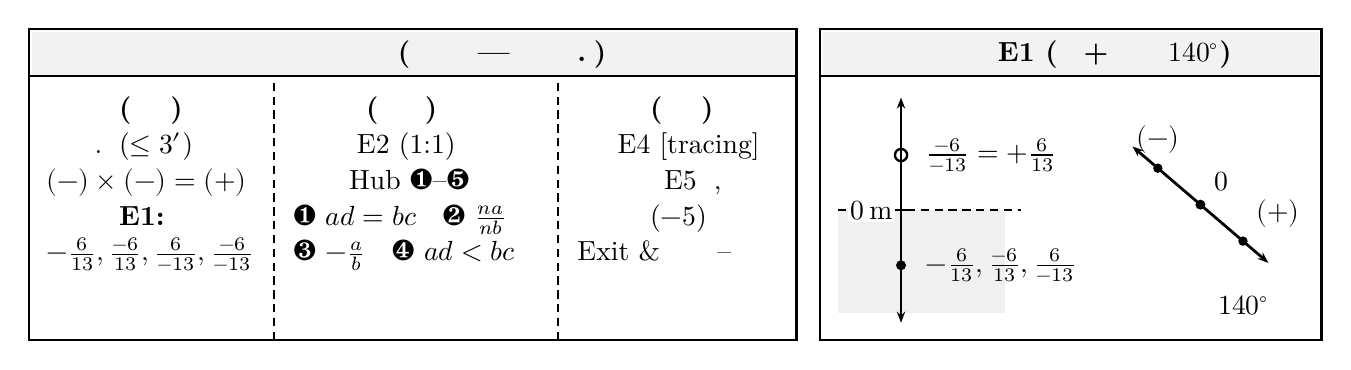
\begin{tikzpicture}[x=0.98cm, y=1cm, every node/.style={font=\linespread{1.0}\fontsize{10pt}{13pt}\selectfont, text=black}]
  % ឆ្វេង៖ ប្លង់ក្ដារខៀន ៣ តំបន់ (0..9.95)
  \draw[black, line width=1.0pt] (0,0) rectangle (9.95,3.95);
  \fill[headgray] (0.04,3.35) rectangle (9.91,3.91);
  \draw[black, line width=0.7pt] (0,3.35) -- (9.95,3.35);
  \node at (4.97,3.63) {\textbf{ប្លង់ក្ដារខៀន ៣ តំបន់ (៥០ នាទី — មេរៀន ២.៣)}};
  \draw[black, densely dashed, line width=0.75pt] (3.18,0) -- (3.18,3.35);
  \draw[black, densely dashed, line width=0.75pt] (6.86,0) -- (6.86,3.35);

  \node[align=left, anchor=north west] at (0.10,3.22) {\textbf{តំបន់ទី១ (ឆ្វេង)}\\ កំណែ ២.២ ($\le 3'$)\\ $(-)\times(-)=(+)$\\ \textbf{បេសកកម្ម \en{E1}:}\\ $-\frac{6}{13}, \frac{-6}{13}, \frac{6}{-13}, \frac{-6}{-13}$};
  \node[align=left, anchor=north west] at (3.30,3.22) {\textbf{តំបន់ទី២ (កណ្ដាល)}\\ ពិសោធន៍ \en{E2} (\en{1:1})\\ ផ្ទាំង \en{Hub} \cnum{1}--\cnum{5}\\ \cnum{1} $ad=bc$ \; \cnum{2} $\frac{na}{nb}$\\ \cnum{3} $-\frac{a}{b}$ \; \cnum{4} $ad<bc$};
  \node[align=left, anchor=north west] at (6.98,3.22) {\textbf{តំបន់ទី៣ (ស្ដាំ)}\\ គំរូ \en{E4} \en{[tracing]}\\ ប្រតិបត្តិ \en{E5} ក, ខ\\ លំហាត់ ១ ($-5$)\\ \en{Exit} \& ផ្ទះ ក--ខ};

  % ស្ដាំ៖ បង្គោលវាស់ទឹក + អ័ក្សផ្អៀង 140 ដឺក្រេ (10.25..16.75)
  \draw[black, line width=0.85pt] (10.25,0) rectangle (16.75,3.95);
  \fill[headgray] (10.29,3.35) rectangle (16.71,3.91);
  \draw[black, line width=0.7pt] (10.25,3.35) -- (16.75,3.35);
  \node at (13.50,3.63) {\textbf{គំនូសបំផុស \en{E1} (ឈរ + ផ្អៀង $140^\circ$)}};

  \fill[panelgray] (10.48,0.35) rectangle (12.65,1.65);
  \draw[black, densely dashed, line width=0.8pt] (10.48,1.65) -- (12.85,1.65);
  \draw[{Stealth[length=4pt]}-{Stealth[length=4pt]}, black, line width=1.05pt] (11.30,0.22) -- (11.30,3.08);
  \draw[black, line width=0.9pt] (11.18,1.65) -- (11.42,1.65) node[left=5pt, fill=white, inner sep=1pt] {$0\unit{m}$};
  \fill[black] (11.30,0.95) circle (1.8pt);
  \node[right=4pt] at (11.35,0.95) {$-\frac{6}{13},\frac{-6}{13},\frac{6}{-13}$};
  \draw[black, line width=0.85pt] (11.30,2.35) circle (2.2pt);
  \node[right=4pt] at (11.35,2.35) {$\frac{-6}{-13}=+\frac{6}{13}$};

  \begin{scope}[shift={(15.18,1.72)}]
    \draw[{Stealth[length=4pt]}-{Stealth[length=4pt]}, black, line width=1.0pt] (140:1.15) -- (-40:1.15);
    \fill[black] (0,0) circle (1.8pt) node[above right=2pt] {$0$};
    \fill[black] (140:0.72) circle (1.7pt) node[above=2pt] {$(-)$};
    \fill[black] (-40:0.72) circle (1.7pt) node[above right=2pt] {$(+)$};
    \node at (0,-1.28) {អ័ក្សផ្អៀង $140^\circ$};
  \end{scope}
\end{tikzpicture}\par
\vspace{3pt}
\figcap{\enbf{1}}{ការបែងចែកប្លង់ក្ដារខៀនទាំង ៣ តំបន់ និងគំនូសបង្គោលវាស់ទឹកស្ពានកំពង់ស្វាយភ្ជាប់អ័ក្សផ្អៀង $140^\circ$ សម្រាប់ \en{E1} \en{(Barrera-Mora \& Reyes-Rodriguez, 2019; Yetim \& Alkan, 2013)}។}
\end{tcolorbox}

ការរៀបចំប្លង់ក្ដារខៀនជា ៣ តំបន់ច្បាស់លាស់ជួយឱ្យគ្រូរក្សាទុកស្លាកបេសកកម្ម \en{E1} នៅតំបន់ទី១ រហូតដល់នាទីទី៤៣ ដើម្បីឱ្យសិស្សផ្ទៀងផ្ទាត់បិទបញ្ចប់បេសកកម្មដោយខ្លួនឯង ខណៈតំបន់ទី២ រក្សាផ្ទាំងធនាគារហេតុផល \cnum{1}--\cnum{5} ជាប់ជានិច្ចសម្រាប់ជាគោលយោងក្នុង \en{E4} និង \en{E5}។

% --- រូបទី ២ ---
\begin{tcolorbox}[enhanced, sharp corners, colback=white, colframe=black, boxrule=0.85pt, top=5pt, bottom=5pt, left=6pt, right=6pt, before skip=4pt, after skip=4pt]
\centering
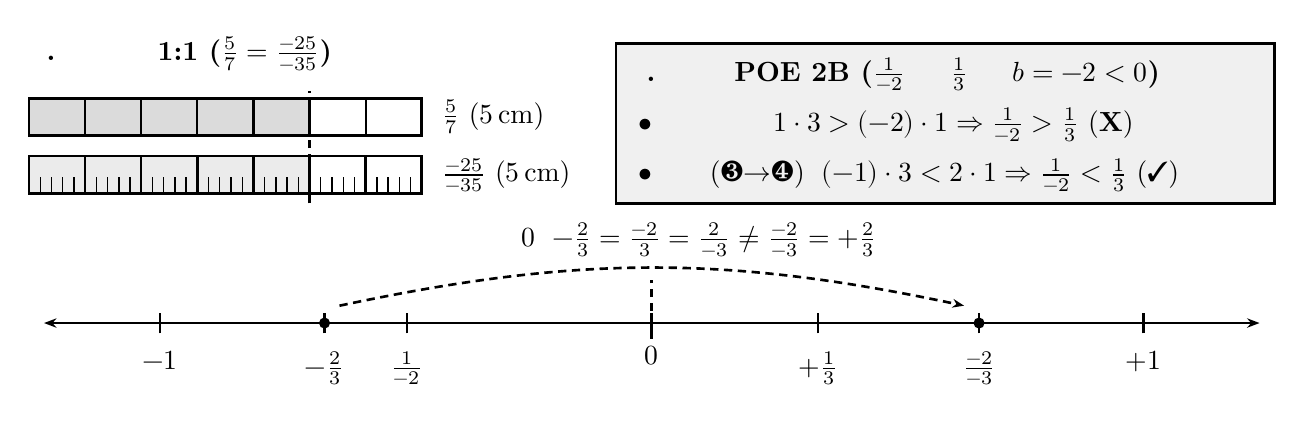
\begin{tikzpicture}[x=0.95cm, y=1cm, every node/.style={font=\linespread{1.0}\fontsize{10pt}{13pt}\selectfont, text=black}]
  % ឆ្វេងលើ៖ បន្ទះប្រភាគសមមូល 5/7 = -25/-35 (y = 2.00..3.95)
  \node[anchor=west] at (0,3.82) {\textbf{ក. បន្ទះសមមូល \en{1:1} ($\frac{5}{7}=\frac{-25}{-35}$)}};
  \fill[gray!28] (0,2.78) rectangle (3.75,3.25);
  \draw[black, line width=1.0pt] (0,2.78) rectangle (5.25,3.25);
  \foreach \k in {1,...,6} { \draw[black, line width=0.8pt] ({0.75*\k},2.78) -- ({0.75*\k},3.25); }
  \node[right=3pt] at (5.28,3.02) {$\frac{5}{7}$ ($5\unit{cm}$)};

  \fill[gray!16] (0,2.05) rectangle (3.75,2.52);
  \draw[black, line width=1.0pt] (0,2.05) rectangle (5.25,2.52);
  \foreach \k in {1,...,6} { \draw[black, line width=0.85pt] ({0.75*\k},2.05) -- ({0.75*\k},2.52); }
  \foreach \m in {1,...,34} { \draw[black, line width=0.5pt] ({0.15*\m},2.05) -- ({0.15*\m},2.25); }
  \draw[black, densely dashed, line width=0.9pt] (3.75,1.92) -- (3.75,3.35);
  \node[right=3pt] at (5.28,2.28) {$\frac{-25}{-35}$ ($5\unit{cm}$)};

  % ស្ដាំលើ៖ POE 2B អន្ទាក់ភាគបែងអវិជ្ជមាន (y = 1.92..3.95)
  \draw[black, line width=0.85pt, fill=panelgray] (7.85,1.92) rectangle (16.65,3.95);
  \node[anchor=west] at (8.02,3.56) {\textbf{ខ. អន្ទាក់ \en{POE 2B} ($\frac{1}{-2}$ ធៀប $\frac{1}{3}$ ពេល $b=-2<0$)}};
  \node[anchor=west] at (8.02,2.92) {$\bullet$ ខុស៖ គុណខ្វែង $1\cdot 3 > (-2)\cdot 1 \Rightarrow \frac{1}{-2}>\frac{1}{3}$ (\enbf{X})};
  \node[anchor=west] at (8.02,2.28) {$\bullet$ ត្រូវ (\cnum{3}$\to$\cnum{4})៖ $(-1)\cdot 3 < 2\cdot 1 \Rightarrow \frac{1}{-2}<\frac{1}{3}$ (\ding{51})};

  % ខាងក្រោមដាច់ស្រឡះ៖ បន្ទាត់ចំនួនឆ្លុះគល់ 0 (POE 2A, y = -0.35..1.45)
  \draw[{Stealth[length=4.5pt]}-{Stealth[length=4.5pt]}, black, line width=1.05pt] (0.20,0.40) -- (16.45,0.40);
  \draw[black, densely dashed, line width=0.9pt] (8.32,-0.15) -- (8.32,0.95);
  \foreach \x/\lbl in {1.75/-1, 3.95/-\frac{2}{3}, 5.05/\frac{1}{-2}, 10.55/+\frac{1}{3}, 12.70/\frac{-2}{-3}, 14.90/+1} {
    \draw[black, line width=0.9pt] (\x,0.27) -- (\x,0.53);
    \node[below=3pt] at (\x,0.27) {$\lbl$};
  }
  \draw[black, line width=0.9pt] (8.32,0.27) -- (8.32,0.53);
  \node[below=3pt, fill=white, inner sep=1.5pt] at (8.32,0.27) {$0$};
  \fill[black] (3.95,0.40) circle (2.0pt);
  \fill[black] (12.70,0.40) circle (2.0pt);
  \draw[traceArr] (4.15,0.62) to[bend left=12] node[above=2pt, fill=white, inner sep=1.5pt] {បត់ឆ្លុះគល់ $0$៖ $-\frac{2}{3}=\frac{-2}{3}=\frac{2}{-3} \neq \frac{-2}{-3}=+\frac{2}{3}$} (12.50,0.62);
\end{tikzpicture}\par
\vspace{3pt}
\figcap{\enbf{2}}{ការគួបផ្សំបន្ទះប្រភាគសមមូល \en{1:1} បន្ទាត់ចំនួនឆ្លុះគល់ $0$ (\en{POE 2A}) និងអន្ទាក់ភាគបែងអវិជ្ជមាន (\en{POE 2B}) លើទំព័រទី១ \en{(Tucker, 2014; Ertuna \& Toluk Uçar, 2021; Çetin, 2022)}។}
\end{tcolorbox}

នៅពេលដឹកនាំ \en{E2} គ្រូគួរឱ្យសិស្សម្នាក់ក្នុងក្រុមបត់សន្លឹកទំព័រទី១ តាមបន្ទាត់ដាច់ៗត្រង់គល់ $0$ ឆ្លុះទៅមុខពន្លឺ ដើម្បីឃើញច្បាស់ថាចំណុច $-\frac{2}{3}$ និង $+\frac{2}{3}=\frac{-2}{-3}$ ស្ថិតនៅម្ខាងម្នាក់នៃគល់ $0$ មានចម្ងាយ $4.00\unit{cm}$ ស្មើគ្នាបេះបិទ។ ការពិសោធដោយដៃនេះលុបបំបាត់ការយល់ច្រឡំសញ្ញាដកពីរជាន់បានយ៉ាងឆាប់រហ័ស។

% --- រូបទី ៣ ---
\begin{tcolorbox}[enhanced, sharp corners, colback=white, colframe=black, boxrule=0.85pt, top=4pt, bottom=4pt, left=6pt, right=6pt, before skip=3pt, after skip=3pt]
\centering
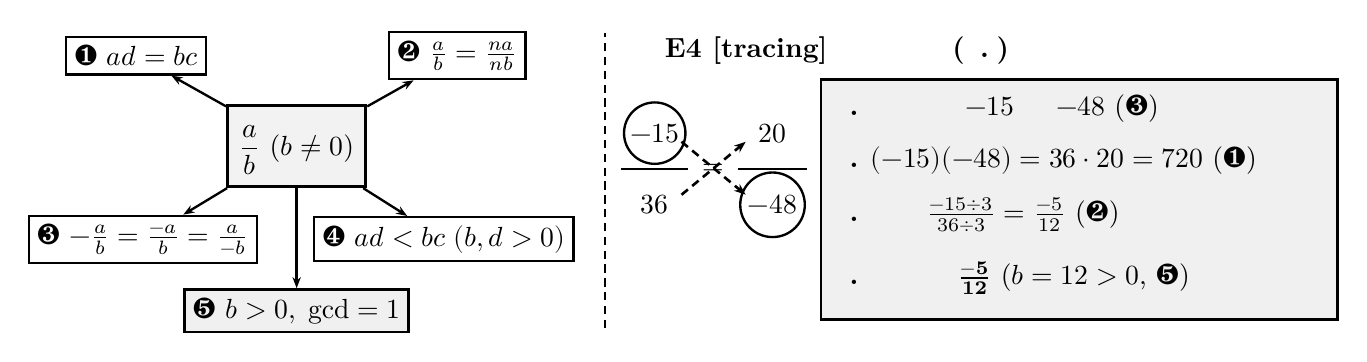
\begin{tikzpicture}[x=0.85cm, y=0.91cm, every node/.style={font=\linespread{1.0}\fontsize{10pt}{13pt}\selectfont, text=black}]
  % ឆ្វេង៖ Hub-and-Spoke ធនាគារហេតុផល 1-5 (0..8.3)
  \node[draw=black, line width=1.05pt, fill=headgray, inner sep=4.2pt, align=center] (hub) at (3.95,1.92)
    {\textbf{ស្នូលសនិទាន}\\[1pt] $\dfrac{a}{b}$ ($b\neq 0$)};
  \node[draw=black, line width=0.8pt, fill=white, inner sep=3.0pt] (s1) at (1.55,3.18) {\cnum{1} $ad=bc$};
  \node[draw=black, line width=0.8pt, fill=white, inner sep=3.0pt] (s2) at (6.35,3.18) {\cnum{2} $\frac{a}{b}=\frac{na}{nb}$};
  \node[draw=black, line width=0.8pt, fill=white, inner sep=3.0pt] (s3) at (1.65,0.62) {\cnum{3} $-\frac{a}{b}=\frac{-a}{b}=\frac{a}{-b}$};
  \node[draw=black, line width=0.8pt, fill=white, inner sep=3.0pt] (s4) at (6.15,0.62) {\cnum{4} $ad<bc\;(b,d>0)$};
  \node[draw=black, line width=0.85pt, fill=panelgray, inner sep=3.0pt] (s5) at (3.95,-0.38) {\cnum{5} $b>0,\;\gcd=1$};
  \foreach \t in {s1,s2,s3,s4,s5} { \draw[black, line width=0.85pt, -{Stealth[length=4pt]}] (hub) -- (\t); }

  \draw[black, densely dashed, line width=0.75pt] (8.55,-0.62) -- (8.55,3.50);

  % ស្ដាំ៖ កាតស៊ើបអង្កេត E4 [tracing] លើលំហាត់គំរូ គ (8.75..19.10)
  \node[anchor=west] at (8.80,3.25) {\textbf{កាត \en{E4 [tracing]}៖ លំហាត់គំរូ គ (ទំ.៥)}};
  \node at (9.30,2.10) {$-15$};
  \draw[black, line width=0.85pt] (9.30,2.10) circle (0.39cm);
  \draw[black, line width=0.95pt] (8.80,1.60) -- (9.80,1.60);
  \node at (9.30,1.10) {$36$};

  \node at (10.18,1.60) {$=$};

  \node at (11.06,2.10) {$20$};
  \draw[black, line width=0.95pt] (10.54,1.60) -- (11.58,1.60);
  \node at (11.06,1.10) {$-48$};
  \draw[black, line width=0.85pt] (11.06,1.10) circle (0.41cm);

  \draw[traceArr] (9.70,1.98) -- (10.66,1.24);
  \draw[traceArr] (9.70,1.24) -- (10.66,1.98);

  \draw[black, line width=0.85pt, fill=panelgray] (11.78,-0.50) rectangle (19.50,2.85);
  \node[anchor=west] at (11.95,2.44) {\textbf{១.} ព័ទ្ធរង្វង់ $-15$ និង $-48$ (\cnum{3})};
  \node[anchor=west] at (11.95,1.72) {\textbf{២.} $(-15)(-48)=36\cdot 20=720$ (\cnum{1})};
  \node[anchor=west] at (11.95,0.96) {\textbf{៣.} សម្រួល $\frac{-15\div 3}{36\div 3}=\frac{-5}{12}$ (\cnum{2})};
  \node[anchor=west] at (11.95,0.08) {\textbf{៤.} បង្រួមរួច៖ $\mathbf{\frac{-5}{12}}$ ($b=12>0$, \cnum{5})};
\end{tikzpicture}\par
\vspace{2pt}
\figcap{\enbf{3}}{រចនាសម្ព័ន្ធគំនិត \en{Hub-and-Spoke} (\cnum{1}--\cnum{5}) និងសញ្ញាសម្គាល់ស-ខ្មៅ \en{[tracing]} លើលំហាត់គំរូ គ \en{(Xu et al., 2026; Yeo \& Tzeng, 2019; Barbieri et al., 2022)}។}
\end{tcolorbox}

ដោយសារសន្លឹកកិច្ចការសិស្សបោះពុម្ពជាស-ខ្មៅ ១០០\% ការឱ្យសិស្សប្រើខ្មៅដៃ \textbf{ព័ទ្ធរង្វង់ជុំវិញតួអវិជ្ជមាន} ($-15$ និង $-48$) មុនពេលអូសម្រាមដៃខ្វែង \en{[tracing]} ជួយជំនួសការប្រើហ្វឺតពណ៌បានទាំងស្រុង និងការពារកំហុសភ្លេចសញ្ញាដកពេលគុណ $(-15)\times(-48)=+720$។

% --- រូបទី ៤ ---
\begin{tcolorbox}[enhanced, sharp corners, colback=white, colframe=black, boxrule=0.85pt, top=5pt, bottom=5pt, left=6pt, right=6pt, before skip=4pt, after skip=4pt]
\centering
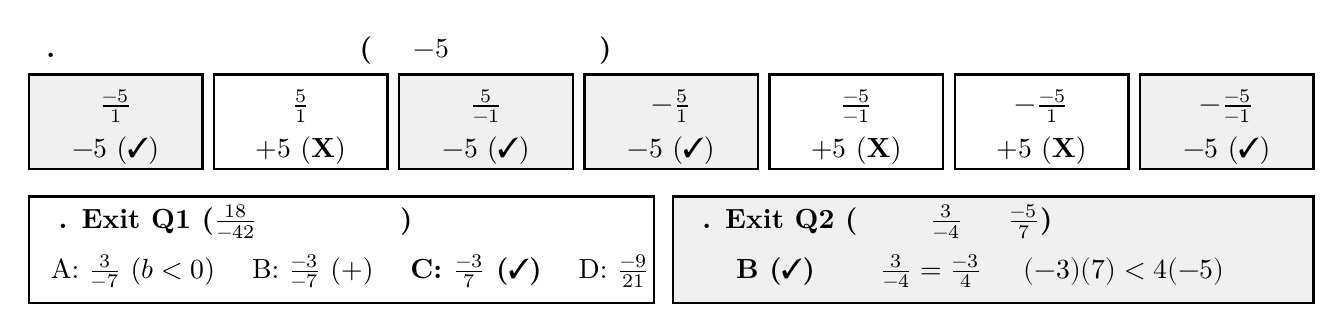
\begin{tikzpicture}[x=0.98cm, y=1cm, every node/.style={font=\linespread{1.0}\fontsize{10pt}{13pt}\selectfont, text=black}]
  % ផ្នែកលើ៖ អ្នកប្រមាញ់តម្លៃ -5 (លំហាត់ ១ ទំព័រ ១១)
  \node[anchor=west] at (0,3.35) {\textbf{ក. ក្បួនរាប់សញ្ញាដកលើលំហាត់ ១ ទំព័រ ១១ (ស្មើ $-5$ ពេលសញ្ញាដកចំនួនសេស)}};
  \foreach \i/\expr/\res/\sh in {
    0/{\frac{-5}{1}}/{-5 \text{ (\ding{51})}}/panelgray,
    1/{\frac{5}{1}}/{+5 \text{ (\enbf{X})}}/white,
    2/{\frac{5}{-1}}/{-5 \text{ (\ding{51})}}/panelgray,
    3/{-\frac{5}{1}}/{-5 \text{ (\ding{51})}}/panelgray,
    4/{\frac{-5}{-1}}/{+5 \text{ (\enbf{X})}}/white,
    5/{-\frac{-5}{1}}/{+5 \text{ (\enbf{X})}}/white,
    6/{-\frac{-5}{-1}}/{-5 \text{ (\ding{51})}}/panelgray} {
    \draw[black, line width=0.85pt, fill=\sh] ({2.40*\i},1.85) rectangle ({2.40*\i+2.25},3.05);
    \node at ({2.40*\i+1.125},2.65) {$\expr$};
    \node at ({2.40*\i+1.125},2.08) {$\res$};
  }

  % ផ្នែកក្រោម៖ Exit Foils Q1 & Q2
  \draw[black, line width=0.85pt, fill=white] (0,0.15) rectangle (8.10,1.50);
  \node[anchor=west] at (0.16,1.18) {\textbf{ខ. \en{Exit Q1} ($\frac{18}{-42}$ បង្រួមរួចស្ដង់ដារ)៖}};
  \node[anchor=west] at (0.16,0.55) {\en{A: $\frac{3}{-7}$ ($b<0$) \quad B: $\frac{-3}{-7}$ ($+$) \quad \textbf{C: $\frac{-3}{7}$ (\ding{51})} \quad D: $\frac{-9}{21}$}};

  \draw[black, line width=0.85pt, fill=panelgray] (8.35,0.15) rectangle (16.65,1.50);
  \node[anchor=west] at (8.50,1.18) {\textbf{គ. \en{Exit Q2} (ប្រៀបធៀប $\frac{3}{-4}$ និង $\frac{-5}{7}$)៖}};
  \node[anchor=west] at (8.50,0.55) {\textbf{បណ្ណ \en{B} (\ding{51})៖} ប្ដូរ $\frac{3}{-4}=\frac{-3}{4}$ រួច $(-3)(7)<4(-5)$};
\end{tikzpicture}\par
\vspace{3pt}
\figcap{\enbf{4}}{ការបែងចែកសញ្ញាដកគូ-សេសក្នុងលំហាត់ ១ (ទំព័រ ១១) និងការវិនិច្ឆ័យជម្រើសអន្ទាក់ក្នុង \en{Exit Foils A--D} \en{(Yetim \& Alkan, 2013; Wesenberg et al., 2022)}។}
\end{tcolorbox}

នៅក្នុងលំហាត់ ១ (ទំព័រ ១១) សិស្សច្រើនភាន់ច្រឡំលើកន្សោមមានសញ្ញាដកបីជាន់ $-\frac{-5}{-1}$ ដោយគិតថាវាស្មើ $+5$។ ការដាក់ប្រអប់ផាត់ប្រផេះលើចម្លើយមានសញ្ញាដកចំនួនសេស ($1$ ឬ $3$ សញ្ញាដក $\Rightarrow -5$) ទល់នឹងប្រអប់ពណ៌សសម្រាប់សញ្ញាដកចំនួនគូ ($0$ ឬ $2$ សញ្ញាដក $\Rightarrow +5$) ជួយឱ្យសិស្សបង្កើតក្បួនទូទៅបានភ្លាមៗ។

\subsec{៤\enbf{.}២ តារាងដោះស្រាយបញ្ហាបន្ទាន់ក្នុងថ្នាក់រៀន \enbf{(Classroom Troubleshooting Guide)}}

\begingroup
\linespread{1.02}\fontsize{10.2pt}{14.6pt}\selectfont
\renewcommand{\arraystretch}{1.12}
\begin{longtable}{|L{3.45cm}|L{4.20cm}|L{2.95cm}|L{6.20cm}|}
\hline
\rowcolor{headgray}
\multicolumn{1}{|C{3.45cm}|}{\tblhead{បញ្ហាប្រឈមក្នុងថ្នាក់}} &
\multicolumn{1}{C{4.20cm}|}{\tblhead{សញ្ញាណសម្គាល់ជាក់ស្ដែង}} &
\multicolumn{1}{C{2.95cm}|}{\tblhead{ប្រភពភស្តុតាង}} &
\multicolumn{1}{C{6.20cm}|}{\tblhead{អន្តរាគមន៍ជួសជុលរហ័សរបស់គ្រូ \enbf{(15--30s)}}} \\
\hline
\endfirsthead
\hline
\rowcolor{headgray}
\multicolumn{1}{|C{3.45cm}|}{\tblhead{បញ្ហាប្រឈមក្នុងថ្នាក់}} &
\multicolumn{1}{C{4.20cm}|}{\tblhead{សញ្ញាណសម្គាល់ជាក់ស្ដែង}} &
\multicolumn{1}{C{2.95cm}|}{\tblhead{ប្រភពភស្តុតាង}} &
\multicolumn{1}{C{6.20cm}|}{\tblhead{អន្តរាគមន៍ជួសជុលរហ័សរបស់គ្រូ \enbf{(15--30s)}}} \\
\hline
\endhead
\hline
\endfoot
\hline
\endlastfoot
\textbf{១. ចែកសញ្ញាដកទៅទាំងលើទាំងក្រោម} & សរសេរ $-\frac{6}{13}=\frac{-6}{-13}$ ឬលើកបណ្ណ \en{B} ($\frac{-3}{-7}$) ក្នុង \en{Exit Q1}។ & \en{Lee \& Boyadzhiev (2020); Yetim \& Alkan (2013)} & ឱ្យមើលបន្ទាត់ចំនួនបត់ឆ្លុះទំព័រ ១ (\en{POE 2A})៖ សញ្ញាដក ២ ចែកគ្នាបានបូក ($+\frac{6}{13}>0$) ខុសសញ្ញាពីចំនួនដើម! \\[3pt]
\hline
\textbf{២. ទុកភាគបែងអវិជ្ជមានក្នុងចម្លើយបង្រួមរួច} & សរសេរទម្រង់បង្រួមរួចជា $\frac{6}{-13}$, $\frac{8}{-15}$ ឬលើកបណ្ណ \en{A} ($\frac{3}{-7}$)។ & \en{Van et al. (2018); Lee \& Boyadzhiev (2020)} & ចង្អុលទៅកាត \cnum{5} លើផ្ទាំងទំព័រ ៤៖ ទម្រង់បង្រួមរួចតម្រូវឱ្យ $b>0$ ដាច់ខាត ត្រូវរុញដកឡើងភាគយកតាម \cnum{3}។ \\[3pt]
\hline
\textbf{៣. គុណខ្វែងវិសមភាពទាំងភាគបែងអវិជ្ជមាន} & គណនា $\frac{3}{-4}$ និង $\frac{-5}{7}$ ដោយយក $3\times 7 > (-4)(-5) \Rightarrow 21>20$ ខុសទិស! & \en{Çetin (2022)} & បង្អាក់ភ្លាមដោយសួរ៖ «តើភាគបែង $-4$ ធំជាង $0$ ឬតូចជាង $0$?» បង្ខំឱ្យប្ដូរជា $\frac{-3}{4}$ តាម \cnum{3} មុនប្រើ \cnum{4}។ \\[3pt]
\hline
\textbf{៤. សម្រួលប្រភាគមិនអស់តួចែករួមធំបំផុត} & សម្រួល $\frac{18}{-42}$ ត្រឹម $\frac{-9}{21}$ (ចែកនឹង $2$) ឬគាំងលើ $\frac{-15}{36}$។ & \en{Jarrah et al. (2022); González-Forte et al. (2021)} & ឱ្យសិស្សពិនិត្យតើ $9$ និង $21$ ចែកដាច់នឹង $3$ ទៀតទេ រួចរំលឹកឱ្យរក $\gcd(18,42)=6$ មុនសម្រួល។ \\[3pt]
\hline
\textbf{៥. វង្វេងលើសញ្ញាដកបីជាន់ក្នុងលំហាត់ ១} & ស្មានខុសថា $-\frac{-5}{-1}=+5$ ឬ $-\frac{-5}{1}=-5$ នៅទំព័រ ១១។ & \en{Yetim \& Alkan (2013)} & ណែនាំឱ្យគិតពីក្នុងប្រភាគចេញក្រៅ៖ $\frac{-5}{-1}=+5$ រួចដាក់សញ្ញាដកខាងមុខបាន $-(+5)=-5$ (សញ្ញាដក ៣ ជាលេខសេស)។ \\[3pt]
\hline
\textbf{៦. បោះពុម្ពទំព័រ ១ ខុសខ្នាត \en{Fit to Page}} & វាស់បន្ទះក្រិតឃើញ $\approx 4.7\unit{cm}$ ជំនួស $5.00\unit{cm}$ ពេលបោះពុម្ព។ & \en{Ertuna \& Toluk Uçar (2021)} & កំណត់ម៉ាស៊ីនព្រីនទៅ \en{Actual Size / 100\%} ជាមុន បើព្រីនរួចហើយឱ្យប្រើក្រិតបន្ទាត់លើក្រដាសផ្ទាល់សម្រាប់ផ្ទឹមសមមូល។ \\[3pt]
\hline
\end{longtable}
\endgroup

% ============================================================================
% ផ្នែកទី ៥៖ មគ្គុទ្ទេសក៍រៀបចំសម្ភារៈបោះពុម្ព (Pages 1--6) និងចម្លើយគំរូពេញលេញ
% ============================================================================
\secbanner{ផ្នែកទី ៥៖ ការរៀបចំសម្ភារៈបោះពុម្ព \enbf{(Pages 1--6)} និងចម្លើយគំរូពេញលេញ}{Section 5: Monochrome Print Preparation (Actual Size 100\%) \& Complete Master Answer Keys}

\subsec{៥\enbf{.}១ ស្តង់ដារបោះពុម្ព \enbf{Actual Size 100\%} និងបរិមាណបោះពុម្ពសម្រាប់ថ្នាក់ ៤០ នាក់}

\begin{enumerate}[leftmargin=0.65cm]
  \item \textbf{ទំព័រទី ១ (បន្ទះ \en{E2} ខ្នាតពិត \en{1:1} — ១០ សន្លឹកសម្រាប់ ១០ ក្រុម)៖} ត្រូវជ្រើស \textbf{\en{Scale: Actual Size 100\%}} (\textit{ហាមជ្រើស \en{Fit to Page}}) ហើយយកបន្ទាត់វាស់ផ្ទៀងបន្ទះក្រិត \en{5.00 cm} នៅជ្រុងស្ដាំខាងលើមុនថតចម្លងចែកក្រុម ដើម្បីធានាថាបន្ទះ $\frac{5}{7}$ ($5.00\unit{cm}$ លើ $7.00\unit{cm}$) និងបន្ទាត់ចំនួនឆ្លុះគល់ $0$ ($1\text{ ឯកតា}=6.00\unit{cm}$) ត្រូវខ្នាតពិតឥតល្អៀង។
  \item \textbf{ទំព័រទី ២ និងទី ៦ (ទម្រង់ \en{2-up} សន្សំក្រដាស)៖} ទំព័រទី២ (កាតស៊ើបអង្កេត \en{E4}៖ បោះពុម្ព ១០ សន្លឹក កាត់ពាក់កណ្ដាលបាន ២០ ប័ណ្ណសម្រាប់ ២០ គូ) និងទំព័រទី៦ (ប័ណ្ណកិច្ចការផ្ទះ៖ បោះពុម្ព ២០ សន្លឹក កាត់ពាក់កណ្ដាលបាន ៤០ ប័ណ្ណចែកសិស្សម្នាក់មួយប័ណ្ណ)។
  \item \textbf{ទំព័រទី ៣, ទី ៤ និងទី ៥៖} ទំព័រទី៣ (សន្លឹក \en{Relay E5}៖ ១០ សន្លឹកសម្រាប់ ១០ ក្រុម), ទំព័រទី៤ (ផ្ទាំងធនាគារហេតុផល \cnum{1}--\cnum{5}៖ បោះពុម្ព ១--២ សន្លឹកលើក្រដាសក្រាស់បិទលើក្ដារខៀន), និងទំព័រទី៥ (បណ្ណ \en{Exit Foils A--D}៖ កាត់ផ្នែកកាត \en{A--D} ចែកសិស្សទុកប្រើប្រចាំឆមាស រីឯផ្នែកកូនសោវិនិច្ឆ័យរក្សាទុកសម្រាប់គ្រូបង្រៀន)។
\end{enumerate}

\subsec{៥\enbf{.}២ តារាងចម្លើយគំរូផ្លូវការសម្រាប់គ្រប់សន្លឹកកិច្ចការ និងលំហាត់ \enbf{(Master Answer Key)}}

\begingroup
\linespread{1.02}\fontsize{10.2pt}{14.6pt}\selectfont
\renewcommand{\arraystretch}{1.12}
\begin{longtable}{|L{3.10cm}|L{13.85cm}|}
\hline
\rowcolor{headgray}
\multicolumn{1}{|C{3.10cm}|}{\tblhead{សន្លឹក \enbf{/} លំហាត់}} &
\multicolumn{1}{C{13.85cm}|}{\tblhead{ចម្លើយគំរូផ្លូវការ ជំហានសម្រាយ និងលេខហេតុផល \enbf{(1--5)}}} \\
\hline
\endfirsthead
\hline
\rowcolor{headgray}
\multicolumn{1}{|C{3.10cm}|}{\tblhead{សន្លឹក \enbf{/} លំហាត់}} &
\multicolumn{1}{C{13.85cm}|}{\tblhead{ចម្លើយគំរូផ្លូវការ ជំហានសម្រាយ និងលេខហេតុផល \enbf{(1--5)}}} \\
\hline
\endhead
\hline
\endfoot
\hline
\endlastfoot
\textbf{ទំព័រ ១ (\en{E2})} \newline បន្ទះសមមូល \en{1:1} &
បន្ទះ \en{A} ($\frac{5}{7}$) និងបន្ទះ \en{B} ($\frac{-25}{-35}=\frac{25}{35}$) មានប្រវែងផាត់ស្មើគ្នា $\mathbf{5.00\unit{cm}}$ លើបន្ទះគោល $7.00\unit{cm}$។ ផ្ទៀងផលគុណខ្វែង៖ $(-25)\times 7 = \mathbf{-175}$ និង $(-35)\times 5 = \mathbf{-175}$ ស្មើគ្នា (\cnum{1}, \cnum{2})។ \\[3pt]
\hline
\textbf{ទំព័រ ១ (\en{E2})} \newline \en{POE 2A \& 2B} &
$\bullet$ \textbf{\en{POE 2A}៖} \textbf{មិនស្មើគ្នា} — $-\frac{2}{3}$ នៅចម្ងាយ $\mathbf{4.00\unit{cm}}$ ខាងឆ្វេង $0$ ឯ $\frac{-2}{-3}=+\frac{2}{3}$ នៅចម្ងាយ $\mathbf{4.00\unit{cm}}$ ខាងស្ដាំ $0$ ព្រោះ $(-)\div(-)=(+)$។ \newline
$\bullet$ \textbf{\en{POE 2B}៖} គុណខ្វែងភ្លាមស្មានខុសថា $>$; លើបន្ទាត់ចំនួនពិត $\frac{1}{-2}$ ($-3\unit{cm}$) $\mathbf{<}$ $\frac{1}{3}$ ($+2\unit{cm}$); មុនគុណខ្វែងត្រូវធ្វើឱ្យភាគបែង \textbf{វិជ្ជមាន ($b>0, d>0$)} ជាមុនសិន (\cnum{3}$\to$\cnum{4})។ \\[3pt]
\hline
\textbf{ទំព័រ ២ (\en{E4})} \newline លំហាត់គំរូ (ទំ.៥) &
$\bullet$ \textbf{ក.} $6\times 13 = \mathbf{78}$ និង $(-13)\times(-6) = \mathbf{78} \Rightarrow \frac{6}{-13}=\frac{-6}{13}$ (\cnum{1}); ទម្រង់បង្រួមរួច៖ $\mathbf{\frac{-6}{13}}$ (\cnum{3}, \cnum{5})។ \newline
$\bullet$ \textbf{ខ.} $\frac{-25}{-35}=\frac{(-5)\times\mathbf{5}}{(-5)\times\mathbf{7}}=\frac{5}{7}$ (\cnum{2}); ទម្រង់បង្រួមរួច៖ $\mathbf{\frac{5}{7}}$ (\cnum{5})។ \newline
$\bullet$ \textbf{គ.} $(-15)\times(-48)=\mathbf{720}$ និង $36\times 20=\mathbf{720} \Rightarrow \frac{-15}{36}=\frac{20}{-48}$ (\cnum{1}); សម្រួល $\frac{-15\div 3}{36\div 3}=\mathbf{\frac{-5}{12}}$ (\cnum{2}, \cnum{5})។ \newline
$\bullet$ \textbf{\en{EIA}៖} សម្រួលមុនបាន $\frac{-5}{12}$ ដូចគ្នាភ្លាម ចំណេញពេល លេខតូច និងមិនងាយខុសគុណលេខធំ $720$។ \\[3pt]
\hline
\textbf{ទំព័រ ៣ (\en{E5})} \newline ប្រតិបត្តិ (ទំ.៥) &
$\bullet$ \textbf{ក.} តួនាទី១៖ $\frac{16}{-30}=\mathbf{\frac{-16}{30}}$ (\cnum{3}); តួនាទី២៖ $16\times 15 = (-30)\times(-8) = \mathbf{240}$ (\cnum{1}); តួនាទី៣៖ សម្រួលនឹង $\gcd=2$ បានទម្រង់បង្រួមរួច $\mathbf{\frac{-8}{15}}$ ($b=15>0$ \ding{51}, \cnum{5})។ \newline
$\bullet$ \textbf{ខ.} តួនាទី១៖ $\frac{-15}{-35}=\mathbf{\frac{15}{35}}$ (\cnum{2}/\cnum{3}); តួនាទី២៖ $\frac{15\div 5}{35\div 5}=\mathbf{\frac{3}{7}}$ និង $\frac{21\div 7}{49\div 7}=\mathbf{\frac{3}{7}}$ (\cnum{2}); តួនាទី៣៖ ទម្រង់បង្រួមរួចគឺ $\mathbf{\frac{3}{7}}$ ($b=7>0$ \ding{51}, \cnum{5})។ \\[3pt]
\hline
\textbf{ទំព័រ ៣ (\en{E5})} \newline លំហាត់ ១ (ទំ.១១) \newline \& បិទ \en{E1} &
$\bullet$ \textbf{លំហាត់ ១ (ទំ.១១)៖} ចំនួនស្មើ $-5$ មាន \textbf{៤ ចំនួន} (សញ្ញាដកចំនួន\textbf{សេស}) គឺ $\mathbf{\frac{-5}{1},\; \frac{5}{-1},\; -\frac{5}{1},\; -\frac{-5}{-1}}$; ចំណែក $\frac{5}{1}, \frac{-5}{-1}, -\frac{-5}{1}$ ស្មើ $+5$។ \newline
$\bullet$ \textbf{បិទ \en{E1}៖} ស្លាកក្រោម $0\unit{m}$ ដូចគ្នាគឺ $\mathbf{-\frac{6}{13}, \frac{-6}{13}, \frac{6}{-13}}$ (\cnum{3}); ស្លាកច្រឡំទៅលើ $0\unit{m}$ គឺ $\mathbf{\frac{-6}{-13} = +\frac{6}{13}}$។ \\[3pt]
\hline
\textbf{ទំព័រ ៥ (\en{E5})} \newline \en{Exit Foils A--D} &
$\bullet$ \textbf{សំណួរទី ១ ($\frac{18}{-42}$)៖} ចម្លើយត្រឹមត្រូវគឺ \textbf{បណ្ណ \en{C} ($\frac{-3}{7}$)} ($\gcd(18,42)=6$ និង $b=7>0$, \cnum{2}+\cnum{3}+\cnum{5})។ \newline
$\bullet$ \textbf{សំណួរទី ២ ($\frac{3}{-4}$ និង $\frac{-5}{7}$)៖} ចម្លើយត្រឹមត្រូវគឺ \textbf{បណ្ណ \en{B}} (ប្ដូរ $\frac{3}{-4}=\frac{-3}{4}$ មុន រួច $(-3)\times 7 = -21 < 4\times(-5)=-20 \Rightarrow \frac{3}{-4}<\frac{-5}{7}$ តាម \cnum{3}$\to$\cnum{4})។ \\[3pt]
\hline
\textbf{ទំព័រ ៦ (ជំហាន ៥)} \newline កិច្ចការផ្ទះ ក.១--២ &
$\bullet$ \textbf{ក.១ ($\frac{-18}{45}, \frac{14}{-35}$)៖} $(-18)\times(-35)=630$ និង $45\times 14=630$ ស្មើគ្នា (\cnum{1}); សម្រួលនឹង $9$ (ឬ $7$) បានទម្រង់បង្រួមរួច $\mathbf{\frac{-2}{5}}$ (\cnum{2}, \cnum{3}, \cnum{5})។ \newline
$\bullet$ \textbf{ក.២ ($\frac{-24}{-56}, \frac{15}{35}$)៖} សម្រួល $\frac{-24}{-56}=\frac{(-8)\times 3}{(-8)\times 7}=\frac{3}{7}$ និង $\frac{15}{35}=\frac{5\times 3}{5\times 7}=\frac{3}{7}$ ស្មើគ្នា (\cnum{2}); ទម្រង់បង្រួមរួចគឺ $\mathbf{\frac{3}{7}}$ (\cnum{5})។ \\[3pt]
\hline
\textbf{ទំព័រ ៦ (ជំហាន ៥)} \newline កិច្ចការផ្ទះ ខ.១--២ &
$\bullet$ \textbf{ខ.១ (ស្មើ $-7$)៖} មាន ៣ ចំនួនគឺ $\mathbf{-\frac{7}{1},\; \frac{7}{-1},\; -\frac{-7}{-1}}$ (ឯ $\frac{-7}{-1}$ និង $-\frac{-7}{1}$ ស្មើ $+7$)។ \newline
$\bullet$ \textbf{ខ.២ (ប្រៀបធៀប $\frac{5}{-8}$ និង $\frac{-3}{5}$)៖} ជំហានទី១ ប្ដូរ $\frac{5}{-8}=\mathbf{\frac{-5}{8}}$ ($b=8>0, d=5>0$ តាម \cnum{3}); ជំហានទី២ គុណខ្វែង $(-5)\times 5 = -25$ និង $8\times(-3) = -24$; ដោយ $-25 < -24$ តាម \cnum{4} បាន $\mathbf{\frac{5}{-8} < \frac{-3}{5}}$។ \\[3pt]
\hline
\end{longtable}
\endgroup

% ============================================================================
% ឯកសារយោង (APA 7th Edition) និងហត្ថលេខា
% ============================================================================
\refbanner{ឯកសារយោង}

{\TimesEn\linespread{1.0}\selectfont\fontsize{10.8pt}{16.2pt}\selectfont
\setlength{\parskip}{3.8pt}
\everypar={\hangindent=0.85cm \hangafter=1}

Alibali, M. W., \& Sidney, P. G. (2015). Variability in the natural number bias: Who, when, how, and why. \textit{Learning and Instruction}, \textit{37}, 56--61. \url{https://doi.org/10.1016/j.learninstruc.2015.01.003}

Barbieri, C. A., Booth, J. L., \& Chawla, K. (2022). Let's be rational: Worked examples supplemented textbooks improve conceptual and fraction knowledge. \textit{Educational Psychology}, \textit{42}(10), 1245--1265. \url{https://doi.org/10.1080/01443410.2022.2144142}

Barrera-Mora, F., \& Reyes-Rodriguez, A. (2019). Fostering middle school students' number sense through contextualized tasks. \textit{International Electronic Journal of Elementary Education}, \textit{12}(1), 75--85. \url{https://doi.org/10.26822/iejee.2019155339}

Çetin, Ö. F. (2022). The awareness of difficulties in solving rational inequality and a solution proposal. \textit{Pedagogical Research}, \textit{7}(4), Article em0137. \url{https://doi.org/10.29333/pr/12392}

Ertuna, L., \& Toluk Uçar, Z. (2021). An investigation of elementary school 4--7th grade students' ability to link equivalent fractions' symbolic and graphical representations. \textit{Sakarya University Journal of Education}, \textit{11}(3), 613--631. \url{https://doi.org/10.19126/suje.992377}

González-Forte, J. M., Fernández, C., Van Hoof, J., \& Van Dooren, W. (2021). Profiles in understanding operations with rational numbers. \textit{Mathematical Thinking and Learning}, \textit{24}(3), 230--250. \url{https://doi.org/10.1080/10986065.2021.1882287}

Jarrah, A. M., Wardat, Y., \& Gningue, S. (2022). Misconception on addition and subtraction of fractions in seventh-grade middle school students. \textit{Eurasia Journal of Mathematics, Science and Technology Education}, \textit{18}(6), Article em2115. \url{https://doi.org/10.29333/ejmste/12070}

Lee, H.-J., \& Boyadzhiev, I. (2020). Underprepared college students' understanding of and misconceptions with fractions. \textit{International Electronic Journal of Mathematics Education}, \textit{15}(3), Article em0583. \url{https://doi.org/10.29333/iejme/7835}

Tucker, S. I. (2014). REFractions: The representing equivalent fractions game. \textit{Australian Primary Mathematics Classroom}, \textit{19}(1), 29--34. (ERIC Document No. EJ1093248). \url{https://files.eric.ed.gov/fulltext/EJ1093248.pdf}

Van, L., Mao, S., \& Cnudde, V. (2018). Improving pedagogical content knowledge on rational numbers of Cambodian teacher trainers. \textit{Global Education Review}, \textit{5}(3), 196--211. \url{https://ger.mercy.edu/index.php/ger/article/download/426/357}

Wesenberg, L., Krieglstein, F., Jansen, S., Rey, G. D., Beege, M., \& Schneider, S. (2022). The influence of the order and congruency of correct and erroneous worked examples on learning and (meta-)cognitive load. \textit{Frontiers in Psychology}, \textit{13}, Article 1032003. \url{https://doi.org/10.3389/fpsyg.2022.1032003}

Xu, Z., Zou, Y., Jin, C., \& Li, L. (2026). Help students construct a hub-and-spoke cognitive structure: A key pathway to reduce burden and improve quality in mathematics classroom teaching. \textit{Frontiers in Psychology}, \textit{17}, Article 1974303. \url{https://doi.org/10.3389/fpsyg.2026.1974303}

Yeo, L.-M., \& Tzeng, Y.-T. (2019). Tracing effect in the worked examples-based learning: An exploration of individual differences in working memory capacity. \textit{Eurasia Journal of Mathematics, Science and Technology Education}, \textit{15}(10), Article em1760. \url{https://doi.org/10.29333/ejmste/105482}

Yetim, S., \& Alkan, R. (2013). How middle school students deal with rational numbers? A mixed methods research study. \textit{Eurasia Journal of Mathematics, Science \& Technology Education}, \textit{9}(2), 213--221. \url{https://doi.org/10.12973/eurasia.2013.9211a}
\par}

\vspace{12pt}
\Needspace{2.2cm}
\hfill
\begin{minipage}{9.8cm}
  {\centering
    ថ្ងៃចន្ទ ៧កើត ខែកត្តិក ឆ្នាំមមី អដ្ឋស័ក ពុទ្ធសករាជ ២៥៧០\\[2pt]
    កំពង់ស្វាយ, ថ្ងៃទី១៦ ខែវិច្ឆិកា ឆ្នាំ២០២៦\\[3pt]
    {\muol\fontsize{11.5pt}{16.5pt}\selectfont គ្រូបង្រៀន}\par}
  \vspace{32pt}
  \hfill{\muol\fontsize{11.5pt}{16.5pt}\selectfont ហុក ប៊ុនថែន}\hspace*{1.4cm}
\end{minipage}

\end{document}
